% =========================
% Main thesis file (English)
% =========================

\documentclass[a4paper,12pt,twoside,openright]{report}

% --- Encoding & fonts ---
\usepackage[utf8]{inputenc}
\usepackage[T1]{fontenc}
\usepackage{libertinus}
\usepackage{newtxmath} % Times-like math matching well with Libertinus

% --- Language (EN only) ---
\usepackage[english]{babel}

% --- Qr Code ---
\usepackage{qrcode}

% --- Page geometry & typography ---
\usepackage[a4paper,top=2.5cm,bottom=2.5cm,left=3cm,right=3cm]{geometry}
\usepackage[fontsize=12pt]{scrextend}
\usepackage[final]{microtype}

% --- Math, tables, figures, colors ---
\usepackage{amsmath}
\usepackage{booktabs}
\usepackage{graphicx}
\usepackage{float}
\usepackage[dvipsnames,table]{xcolor}

% --- Text / utilities ---
\usepackage{rotating}
\usepackage{ragged2e}
\justifying
\usepackage{url}
\usepackage[normalem]{ulem}
\usepackage{afterpage}
\usepackage{xpatch}
\usepackage{enumitem}
\usepackage{multirow}
\usepackage{longtable}
\usepackage{multicol}
\usepackage{dirtree}

% --- Code listings (prefer minted; requires -shell-escape) ---
\usepackage{listings} % kept for completeness
\usepackage{minted}
\usemintedstyle{manni}
\setminted[typescript]{%
  framesep=2mm,
  baselinestretch=1.2,
  fontsize=\ttfamily\footnotesize,
  linenos
}
% compact minted spacing
\AtBeginEnvironment{minted}{\vspace{-0.5em}}
\AfterEndEnvironment{minted}{\vspace{-0.5em}}

% --- Captions & subfigures ---
\usepackage{caption}
\usepackage{subcaption}
% remove "Table" prefix (as in your original)
\captionsetup[table]{labelformat=empty}

% --- Custom "code" environment for captionable code blocks ---
\newenvironment{code}{\captionsetup{type=listing}}{}

% --- Spacing around floats ---
\setlength{\intextsep}{8pt plus 2pt minus 2pt}
\setlength{\abovecaptionskip}{4pt plus 2pt minus 2pt}
\setlength{\belowcaptionskip}{0pt plus 2pt minus 2pt}
\usepackage[section]{placeins}
\flushbottom
\setlength{\textfloatsep}{8pt plus 2pt minus 2pt}
\setlength{\floatsep}{6pt plus 2pt minus 2pt}

% --- Header / footer ---
\usepackage{fancyhdr}
\pagestyle{fancy}
\fancyhf{}
\lhead{\rightmark}
\rhead{\textbf{\thepage}}
\fancyfoot{}
\setlength{\headheight}{27pt}
\addtolength{\topmargin}{-12pt}
\fancypagestyle{plain}{
  \fancyfoot{}
  \fancyhead{}
  \renewcommand{\headrulewidth}{0pt}
}

% --- TikZ ---
\usepackage{tikz}
\usetikzlibrary{positioning,calc,arrows.meta,decorations.pathreplacing}

% --- Small helper macros ---
\newcommand{\matchQCtablesize}{%
  \small
  \setlength{\tabcolsep}{9pt}%
  \renewcommand{\arraystretch}{1.15}%
}
\newcommand\blankpage{%
  \null
  \thispagestyle{empty}%
  \addtocounter{page}{-1}%
  \newpage
}

% --- Icons next to titles (kept as in your setup) ---
\usepackage{etoolbox}
\newcommand{\icon}[1]{\includegraphics[height=12pt]{#1}}
\robustify{\icon}

% --- Keywords environment (English) ---
\newenvironment{keywords}{%
  \begin{center}
    \textbf{Keywords}\par\vspace{0.5em}
    \begin{minipage}{0.85\textwidth}\small
}{%
    \end{minipage}
  \end{center}
}

% --- Index (if used) ---
\usepackage{makeidx}
\makeindex

% --- Bibliography ---
\usepackage[numbers,sort&compress]{natbib}

% --- Labels in English ---
\addto\captionsenglish{%
  \renewcommand{\contentsname}{Table of Contents}
  \renewcommand{\chaptername}{Chapter}
  \renewcommand{\indexname}{Index}
}

% --- Hyperref LAST ---
\usepackage[colorlinks=true,allcolors=black]{hyperref}

% =========================
% Document
% =========================
\begin{document}
\selectlanguage{english}

\begin{titlepage}

\begin{center}

% --- University header ---
{\huge \textbf{University of Turin}} \\[4pt]
{\Large \textsc{School of Natural Sciences}} \\[2pt]
{\large Bachelor's Degree in Computer Science} \\[8mm]

% --- Logo ---

\includegraphics[keepaspectratio=true,scale=0.4]{images/unito_logo.png} \\[5mm]

\end{center}

\begin{center}
    \LARGE{Bachelor's Thesis}
\end{center}

\vspace{15mm}
\begin{center}
    {\huge\textbf{Generative AI and Machine Learning for Time Series}}
\end{center}
\vspace{30mm}

\begin{minipage}[t]{0.47\textwidth}
	{\large{Supervisor:}{\normalsize\vspace{3mm}
	\bf\\ \large{Prof. Robert René Maria Birke} \normalsize\vspace{3mm}\bf}}
\end{minipage}
\hfill
\begin{minipage}[t]{0.47\textwidth}\raggedleft
	{\large{Candidate:}{\normalsize\vspace{3mm} \bf\\ \large{Federico Santorsola\\1025104}}}
\end{minipage}

\vspace{40 mm}
\hrulefill
\\ \centering{\large{ACADEMIC YEAR 2024/2025}}

\end{titlepage}
% \afterpage{\blankpage}
%\thispagestyle{plain}

%\vspace*{10cm}
%{\raggedleft
%\textit{“Intelligence is the ability to adapt to change.”}\\[0.5em]
%--- \textsc{Stephen Hawking}\par}


\thispagestyle{plain}

\vspace*{0.5\textheight}
\begin{flushright}
\textit{``Intelligence is the ability to adapt to change.''}\\[1em]
--- \textsc{Stephen Hawking}
\end{flushright}
% \afterpage{\blankpage}

\begin{abstract}
Time series are a fundamental component in numerous fields of application. Their analysis requires methodologies capable of handling large volumes of data, preserving temporal accuracy, and efficiently managing problems such as missing values and high variability. Traditional techniques, based on statistical models or classic \textit{forecasting} methods, are often limited when it comes to generating plausible synthetic data, reconstructing missing portions, or simulating alternative scenarios in a manner consistent with the multivariate and seasonal structures of the data. \textit{Diffusion Models} have become one of the most promising methodologies for generating sequential data, as they are capable of processing complex distributions and generating reliable samples. Among these, WaveStitch represents an innovative approach that combines arbitrary conditioning, parallelized generation, and cyclic representation of temporal characteristics, in order to better manage the tasks of imputation, forecasting, and simulation of time series. The results obtained have confirmed the potential of this model as a flexible and efficient tool in contexts characterized by the presence of time series, making it ideal for new research perspectives, but also for practical applications in critical, fragile, or sensitive situations, where reliable synthetic data is essential.
\begin{keywords}
WaveStitch, synthetic generation, diffusion models, time series, data imputation, forecasting, comparative analysis
\end{keywords}
\end{abstract}


% \afterpage{\blankpage}

\thispagestyle{plain}
\vspace*{\fill}
\textit{I declare to be responsible for the content I'm presenting in order to
obtain the final degree, not to have plagiarized in all or part of, the
work produced by others and having cited original sources in consistent
way with current plagiarism regulations and copyright. I am also aware
that in case of false declaration, I could incur in law penalties and my
admission to final exam could be denied.}
\vspace*{\fill}
% \afterpage{\blankpage}

% --- Table of contents ---
\tableofcontents
\cleardoublepage

% --- Chapters ---
% \chapter{Chapter Title}

An introduction here (with a cite from bibliography, like this: \cite{greenwade93}).
%  ----
\section{Type of texts}
\subsection{Normal text}
\lipsum[1]

\subsection{Normal text}
\textbf{\lipsum[1]}

\subsection{Italic text}
\textit{\lipsum[1]}

\subsection{Mono space text}
\subsubsection{(usually I use this type of format to refer me to code)}
\texttt{Here is some text. Pay attention to this type, because It can go 
\\ out of bounds! Usually you solve it with a double back-slash, to 
\\ go to the new line.}
%  ----

%  ----
\section{Lists}
\subsection{Unbulleted lists}
\begin{itemize}
    \item \lipsum[1]
    \item \lipsum[1]
    \item \lipsum[1]
\end{itemize}

\subsection{Bulleted lists}
\begin{enumerate}
    \item \lipsum[1]
    \item \lipsum[1]
    \item \lipsum[1]
\end{enumerate}
%  ----

%  ----
\section{Images}
Random Duolingo Image example:
\begin{figure}[H]
\centering
    
\includegraphics[scale=0.1]{images/duolingo.png}
    \caption{Caption example.}
    \label{fig:duolingo}
\end{figure}

In the text, you reference an image in this way: \ref{fig:duolingo}.
%  ----

%  ----
\section{Tables}
Example of table that can even be split into several pages if it's too long:
\begin{longtable}[H]{| l | l |}
    \hline
     \rowcolor[HTML]{F87C58}\textbf{Head 1} & \textbf{Head 2}\\
    \hline
    \endfirsthead
    
    \texttt{Text} & \texttt{Text}\\
    \hline
    \texttt{text} & \texttt{Text}\\
    \hline
    \texttt{Text} & \texttt{Text}\\
    \hline
    \texttt{text} & \texttt{Text}\\
    \hline
    \texttt{Text} & \texttt{Text}\\
    \hline
    \texttt{text} & \texttt{Text}\\
    \hline
    \texttt{Text} & \texttt{Text}\\
    \hline
    \texttt{text} & \texttt{Text}\\
    \hline
    \texttt{Text} & \texttt{Text}\\
    \hline
    \texttt{text} & \texttt{Text}\\
    \hline
    \texttt{Text} & \texttt{Text}\\
    \hline
    \texttt{text} & \texttt{Text}\\
    \hline
    \texttt{Text} & \texttt{Text}\\
    \hline
    \texttt{text} & \texttt{Text}\\
    \hline
    \texttt{Text} & \texttt{Text}\\
    \hline
    \texttt{text} & \texttt{Text}\\
    \hline
    \texttt{Text} & \texttt{Text}\\
    \hline
    \texttt{text} & \texttt{Text}\\
    \hline
    \texttt{Text} & \texttt{Text}\\
    \hline
    \texttt{text} & \texttt{Text}\\
    \hline
    \caption{Table caption.}
\end{longtable}
%  ----

%  ----
\section{Code}
Finally, here we are with code! The following examples are with typescript and HTML with Angular syntax, colored using the \textbf{minted} package.

\begin{code}
    \inputminted{typescript}{listings/ts-example.ts}
    \caption{Caption for the typescript example.}
\end{code}
\vspace{4mm}

\begin{code}
    \inputminted{ng2}{listings/html-example.html}
    \caption{Caption for the HTML with Angular syntax example.}
\end{code}
\vspace{4mm}
%  ----
\chapter{Introduction and Objectives of the Work}
\label{chap:intro_eng}

The volume of activity carried out by High-Performance Computing (HPC) centres has led to an exponential increase in the amount of data generated and monitored within research institutions and energy infrastructures, for example, data collected by sensors inside the rooms housing the servers.  
This energy and environmental consumption data is a valuable source of information but also potentially sensitive: by analysing power and temperature variations, it is possible to indirectly infer information about system activity, such as workload intensity or peak usage times.  
Access to and sharing of this data are therefore limited by confidentiality and security constraints.  
In this context, the \textbf{generation of realistic synthetic time series} represents a promising solution to reconcile two often conflicting requirements: on the one hand, the need to conduct advanced analyses and develop predictive models; on the other, the protection of privacy and operational security within data centres.  
Creating synthetic data consistent with real data makes it possible to train and validate artificial intelligence models, experiment with optimisation algorithms, and evaluate energy efficiency strategies without exposing confidential information.

\section*{Objective of the Work}

The objective of this work was to \textbf{produce synthetic time series of energy consumption that are realistic and consistent with the real data of the HPC centre in Turin}, using generative artificial intelligence models based on diffusion processes.  
In particular, the project is part of the broader field of research on conditional generation of time series data, in which synthetic sequences are created by taking into account auxiliary variables --- such as rack type, date, time, or other operating conditions --- in order to preserve the original patterns and correlations.

\section*{Approach Followed}

To address the problem, I designed and implemented a complete analysis and modelling workflow, consisting of four main phases:

\begin{enumerate}
  \item \textbf{Data cleaning and normalisation}: collection and cleaning of energy data from InfluxDB, with verification of temporal consistency, removal of outliers, and standardisation of sampling frequencies;
  \item \textbf{Exploratory analysis and clustering}: study of correlations between electrical quantities and identification of recurring operating regimes using \emph{k-Means} and \emph{PCA} techniques;
  \item \textbf{Generative training with \emph{WaveStitch}}: application and adaptation of the \emph{WaveStitch} diffusion model~\cite{wavestitch} for the conditional generation of time series in the HPC energy domain;
  \item \textbf{Real vs synth evaluation and comparison}: analysis of synthetic sequences generated through numerical (\emph{MSE}) and structural (\emph{ACD} and \emph{xCorrDiff}) metrics to verify fidelity and statistical consistency with the original data.
\end{enumerate}
This approach made it possible to build a replicable and scalable workflow, capable of integrating \emph{data preprocessing}, \emph{unsupervised learning}, and \emph{generative artificial intelligence} techniques within a single application framework.

\section*{Main Results}

The results obtained show that, once properly calibrated, the \emph{WaveStitch} model is capable of generating synthetic sequences that are \textbf{consistent, realistic, and statistically aligned} with the real time series of the HPC centre.  
Structural metrics (\emph{Autocorrelation Difference} and \emph{Cross-feature Correlation Difference}) demonstrated high fidelity of temporal and multivariate patterns, while numerical measures (\emph{MSE}) confirmed good point-by-point alignment between real and synthetic traces.
Overall, this work demonstrated how diffusion models can serve as a valid alternative to traditional approaches for data generation and imputation --- in this case, energy data --- contributing to the development of new strategies for \textbf{modelling, simulation, and protection of sensitive data} across a wide range of applications.
\chapter{Theoretical foundations}
% -----------------------------
\section{Diffusion models, WaveStitch, and time series}

\textit{Diffusion} models (DM) represent one of the most recent and promising families of generative models. They operate in two main phases:

\begin{enumerate}
    \item \textbf{Forward process (noising):} Gaussian noise is added to the original sample progressively, step by step, until the distribution is almost completely devoid of the initial information. This process simulates how a noise source can "corrupt" initial data.
    
    \item \textbf{Reverse process (denoising):} a neural network is trained to learn the inverse of the degradation process. Starting from pure noise, it is progressively reduced and the network performs an iterative denoising process that reconstructs plausible samples consistent with the distribution of the real data.
\end{enumerate}
This probabilistic formulation allows complex distributions to be modeled and realistic samples to be generated, and forms the basis of modern \textit{Denoising Diffusion Probabilistic Models} (DDPM) and \textit{score-based} models, which have redefined the state of the art in deep generative models~\cite{sohldickstein2015,ho2020ddpm,song2020score,dhariwal2021improved}.  
\textbf{WaveStitch}~\cite{wavestitch} fits into this trend by introducing an innovative approach to the problem of conditional time series generation. The distinctive feature is the \textit{conditional stitching} mechanism, which allows to:

\begin{itemize}
    \item reconstruct missing values (\textit{imputation});
    \item predict future values (\textit{forecasting});
    \item generate alternative scenarios consistent with real data (\textit{simulation}).
\end{itemize} 

\begin{figure}[H]
\centering
    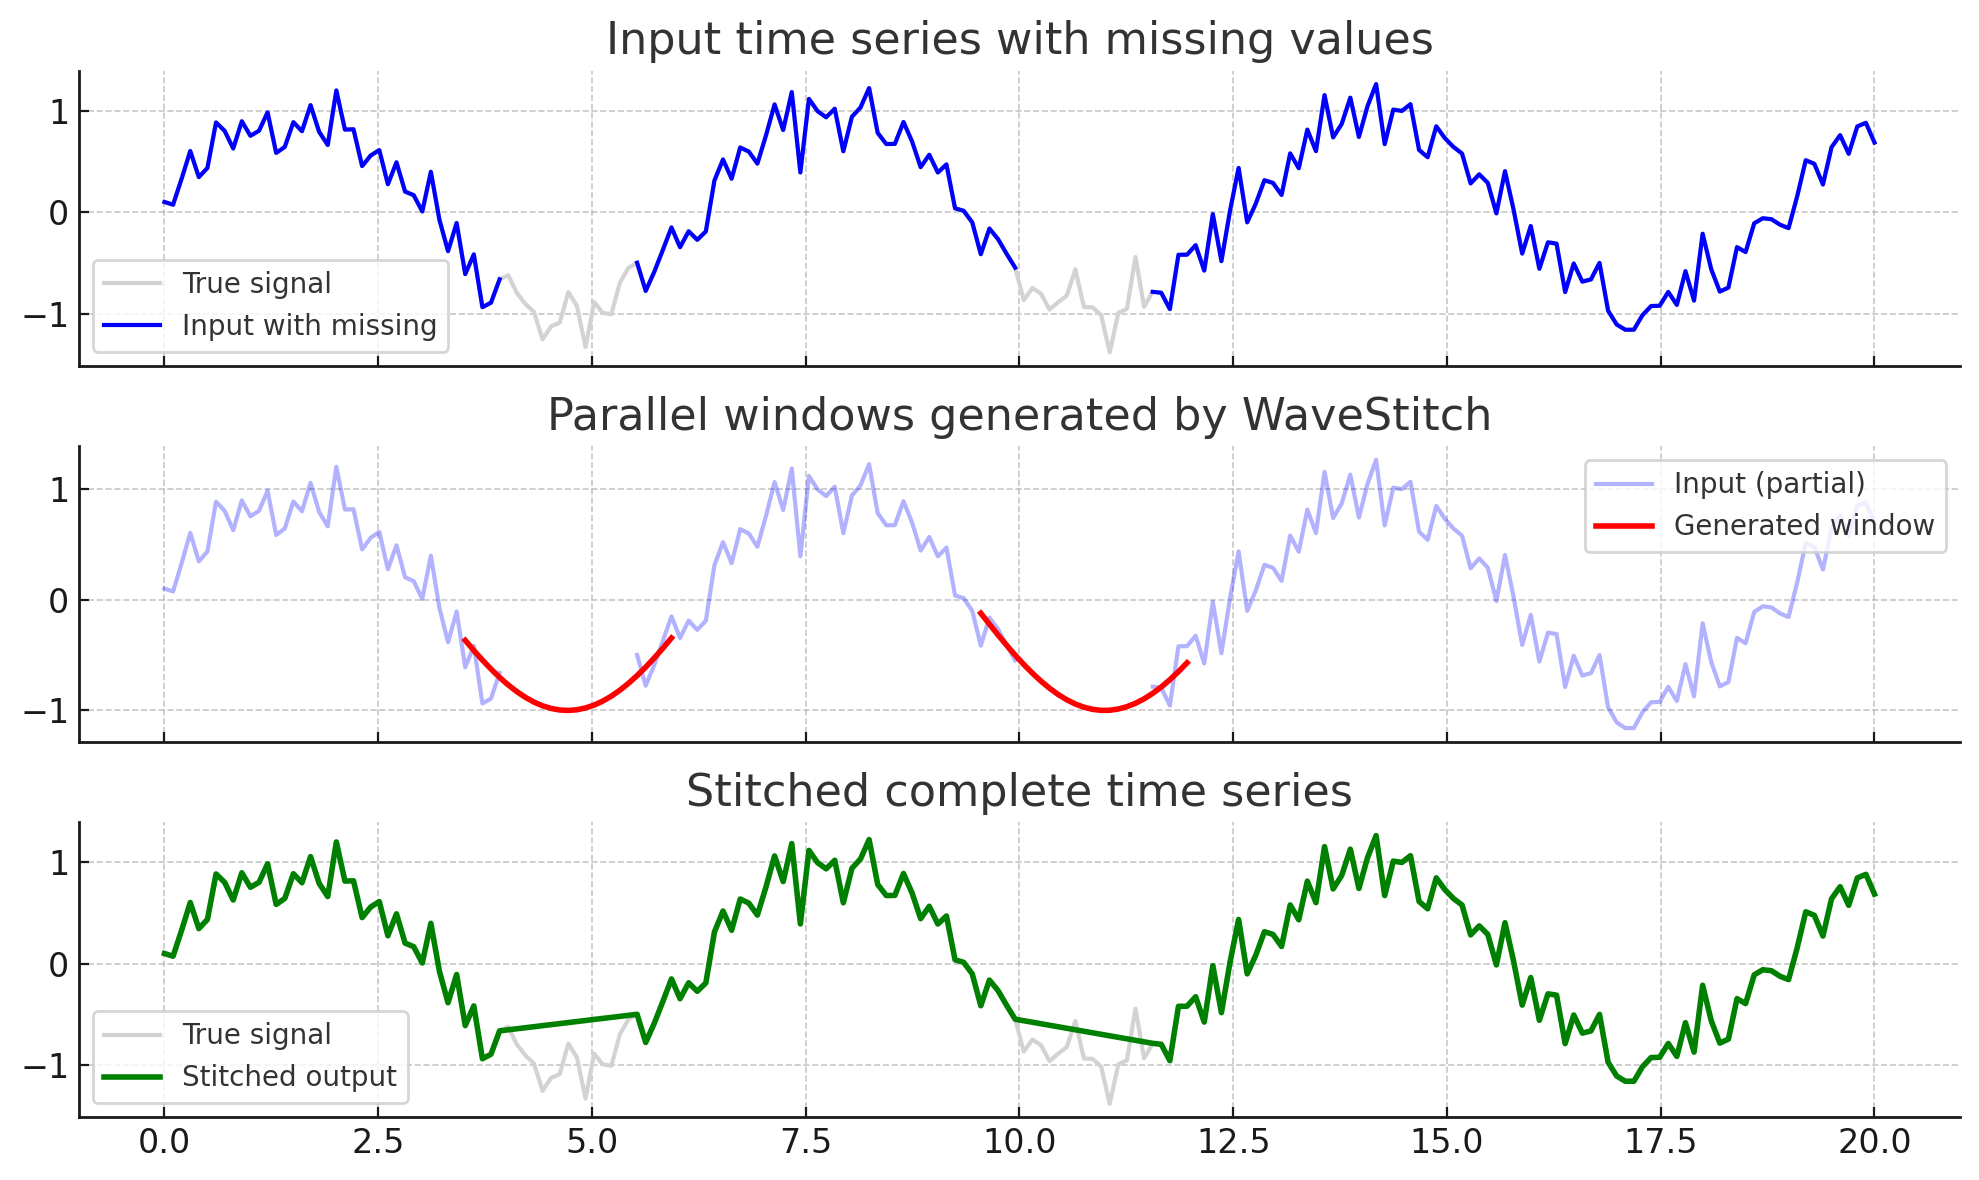
\includegraphics[width=0.75\textwidth]{images/esempio_wavestitch.png}
    \caption{Conceptual diagram of how WaveStitch works (own elaboration): (top) input with missing values; (center) windows generated in parallel; (bottom) complete series obtained through \textit{stitching}.}
    \label{fig:wavestitch_schema}
\end{figure}


% ------------------------
\section{Machine learning in relation to this work}

\textbf{Machine learning} (ML) is now one of the most powerful tools for analyzing and modeling complex data.  
In a nutshell, I would say that the idea behind ML is to train algorithms capable of learning rules and patterns directly from data, without the need for explicit programming.  

% ----------------------
\subsection{Supervised vs. Unsupervised Learning}

I would say that the work I am presenting straddles two classic ML paradigms:

\begin{itemize}
    \item \textbf{Supervised Learning:} there is a model that is trained on a labeled dataset (each instance associated with the corresponding class). This means that for each example in the training dataset, there is a corresponding label or desired result. The goal of the model is to learn a function that maps inputs to the correct outputs, so that it can make accurate predictions on new, unseen data.  

    \item \textbf{Unsupervised learning:} when data does not have explicit labels, classes are not known a priori. In this case, the goal is to identify latent structures or statistical relationships, as occurs when we cluster data.  
\end{itemize}
Although the \emph{WaveStitch} model is a conditional generator, it works in a manner similar to \emph{unsupervised learning}, as it learns the distribution of data without the need for explicit labels, but uses masks and conditional constraints to guide generation.

% ----------------------
\subsection{Mathematical example}

A simple example of a supervised learning model is \textbf{linear regression}, which aims to estimate a linear relationship between a set of independent variables and a dependent variable.  
In compact form, the model can be expressed as:

\[
\hat{y} = w_0 + w_1 x_1 + w_2 x_2 + \dots + w_n x_n,
\]

where \( \hat{y} \) represents the predicted value, \( x_i \) the input variables, and \( w_i \) the associated weights (or coefficients), including the intercept \( w_0 \).  
The model parameters are estimated by minimizing a loss function, typically the \emph{mean squared error} (MSE), defined as:

\[
MSE = \frac{1}{n} \sum_{i=1}^{n} (y_i - \hat{y}_i)^2,
\]

where \( y_i \) is the observed actual value and \( \hat{y}_i \) the corresponding model prediction.  
Minimizing the MSE allows us to obtain the coefficients \( w_i \) that best approximate the relationship between the variables, minimizing the overall difference between actual and estimated values.

\medskip

\noindent
\textbf{WaveStitch}, on the other hand, does not seek a deterministic function \( f(x) \), but learns to generate samples from a probabilistic distribution \( p(x) \), through a process of \emph{diffusion} and subsequent \emph{denoising}~\cite{wavestitch}.  
\emph{Machine learning} therefore acts as a methodological glue between raw data management and the application of advanced generative models, but without adequate \emph{preprocessing} and preliminary statistical analysis, as I will show in the following chapters, even a powerful model such as WaveStitch would fail to produce consistent and reliable results~\cite{bishop2006pattern,hastie2009elements}.
% --------------------------------

\section{Data Clustering in Artificial Intelligence}

\textbf{Clustering} is an \emph{unsupervised learning} technique that allows a set of data to be divided into homogeneous groups, called \emph{clusters}, so that observations belonging to the same group are \emph{similar} to each other, while those belonging to different groups are \emph{dissimilar}~\cite{jain2010data}.  
Clustering is a fundamental tool for exploring and understanding data, as it allows latent structures, recurring patterns, and hidden relationships to be identified without resorting to predefined labels.

\subsection{Basic principles}

Given a set of $n$ objects and a predetermined number $k \leq n$ of clusters to be created, the goal of clustering is to organize the data into $k$ partitions such that:
\begin{itemize}
  \item objects within the same cluster are \textit{similar} to each other;
  \item objects belonging to different clusters are \textit{dissimilar}.
\end{itemize}
In other words, clustering can be considered a form of \emph{lossy data compression}, in which each group represents a collective abstraction of multiple observations.

\subsection{k-Means algorithm}

During my Information Systems course, I learned about various algorithms such as \textbf{k-medoids} and \textbf{k-modes}, but for this work I wanted to choose one of the most widespread and widely used as a tool and subject of study: \textbf{k-Means}. I will explain how it works below.  
The algorithm operates according to an iterative partitioning approach, in which each data point is assigned to the cluster whose \emph{centroid}—i.e., the average of the points belonging to that cluster—is closest.  

The process can be described as follows:
\begin{enumerate}
  \item $k$ initial centroids are randomly selected from the dataset.
  \item Each point is assigned to the cluster with the closest centroid (usually according to Euclidean distance).
  \item The centroids are updated as the average of the points assigned to each cluster.
  \item Steps (2)–(3) are repeated until convergence, i.e., until the assignments do not change or a maximum number of iterations is reached.
\end{enumerate}

Formally, the algorithm minimizes the following objective function:

\[
J = \sum_{i=1}^{k} \sum_{x \in C_i} \| x - \mu_i \|^2
\]

where $C_i$ represents the $i$-th cluster and $\mu_i$ its centroid.  
The aim is therefore to minimize the overall distance of the points from their respective centroids, obtaining compact and well-separated clusters.

\subsection{Advantages and limitations}

The k-Means method has several advantages:
\begin{itemize}
  \item it is simple to implement and conceptually intuitive;
  \item it is scalable and efficient even on large datasets, with complexity $O(nkt)$, where $n$ is the number of objects, $k$ is the number of clusters, and $t$ is the number of iterations;
  \item it works well when clusters are compact and separable.
\end{itemize}

However, it also has some limitations~\cite{jain2010data}:
\begin{itemize}
  \item it requires specifying the number $k$ of clusters in advance;
  \item it is sensitive to the choice of initial centroids and can converge to local optima;
  \item it is not suitable for non-convex clusters or clusters with very different densities;
  \item it is influenced by \emph{outliers}, which can significantly alter the position of the centroids.
\end{itemize}

\subsection{Convergence and variants}

The k-Means algorithm guarantees convergence in a finite number of steps, since there is a finite number of possible data partitions and each iteration reduces (or keeps constant) the objective function $J$. In the next chapter I will talk about the Wavestitch Paper. 

\chapter{WaveStitch: Flexible and Fast Conditional Time Series Generation with Diffusion Models}

\section{Introduction}
As I mentioned, \textbf{Wavestitch} is the diffusion model I have been tasked with researching.  
In this chapter, I would like to provide a general overview of it using the paper that describes it.  
The document begins by showing the three critical issues identified by the authors in the conditional generation of time series—the lack of adaptability of existing models to inference conditions, the slowness of autoregressive generative processes, and inefficiency in the encoding of categorical characteristics—which have been addressed through innovative and efficient solutions: a flexible conditioning mechanism, a parallel generation procedure with segment \emph{stitching}, and cyclic encoding of categorical variables.  
These methodological choices make it possible to overcome the structural limitations of previous models, leading to significant improvements in both accuracy and computational efficiency~\cite{wavestitch} .

\section{Challenges addressed}

\subsection{Q1: Adaptability to inference conditions}S
One of the most significant limitations of existing generative models is their poor ability to adapt to changing conditions during inference.  
In many application contexts, time series depend not only on their historical trends, but also on auxiliary variables or metadata (e.g., year, month, district, type of service).  
Models such as TimeGAN or conditioned LSTM variants are trained on fixed configurations of conditions, which limits their ability to generalize to scenarios never seen during training.  
This rigidity translates into low operational flexibility: if new combinations are required during inference (e.g., a specific year associated with a brand not present in the training), the models are unable to adapt and produce inconsistent or statistically implausible samples~\cite{yoon2019timegan}.

\subsection{Q2: Slowness of autoregressive methods}
Most classical methods for generating time series are \emph{autoregressive} in nature, i.e., they generate values one at a time, using sliding windows.  
While this approach ensures sequential consistency, it comes at a very high computational cost: generation becomes slow and difficult to parallelize, especially when working with large datasets or extended time horizons.  
For real-world applications—such as monitoring energy consumption in an HPC center or managing healthcare data—speed is a fundamental requirement.  
A method that takes minutes or hours to generate a synthetic sequence is impractical, especially when integrated into simulation or \emph{real-time decision-making} systems.  
Consequently, the slowness of sequential methods represents a real obstacle to their industrial adoption~\cite{yoon2019timegan,zhou2023timeweaver}.

\subsection{Q3: Inefficient encoding of categorical features}
Time series are often influenced by categorical features, such as days of the week, months, or codes indicating membership in a certain group of devices.  
The most commonly used method for representing these variables is \emph{one-hot encoding}, which, however, has two main limitations:
\begin{itemize}
    \item it significantly increases the dimensionality of the input, making the model heavier and more difficult to train;
    \item it does not naturally represent the periodicity of variables, such as daily or monthly cycles, where extreme values (e.g., December and January) should be close together but are instead placed at opposite ends of the coding spectrum.
\end{itemize}
This inefficiency in representation results in a loss of structural information, which can compromise the model’s ability to capture cyclical regularities typical of energy, financial, or environmental time series.  
These challenges constitute the motivational context within which WaveStitch was developed, whose architecture aims to provide innovative solutions for each of the problems highlighted~\cite{wavestitch}.

\section{Methodology and proposed solution}

The methodology behind \textbf{WaveStitch} stems from the need to systematically address the three main challenges identified in the previous paragraph.  
The authors propose an architecture that exploits \emph{Denoising Diffusion Probabilistic Models} (DDPMs)~\cite{ho2020ddpm}.

\subsection{Flexible constraint management (Q1)}
The first innovation of WaveStitch concerns its ability to generalize to conditions never seen during training.  
The model is trained in two distinct phases:
\begin{enumerate}
    \item \textbf{Training:} the denoiser is trained to generate a complete signal conditioned \emph{only} on auxiliary characteristics (e.g., year, month, region).  
    \item \textbf{Inference:} at the time of generation, constraints from the actual values of the observed signal (e.g., available portions of the series) are also introduced.  
    Through conditional masks, the model integrates this partial information and produces coherent sequences that comply with both metadata and historical data.  
\end{enumerate}
This approach makes WaveStitch flexible and capable of adapting to unexpected scenarios, such as the request to generate a time series block for combinations of conditions not present in the training dataset~\cite{wavestitch}.

\subsection{Parallel generation with stitching (Q2)}
To solve the problem of slow autoregressive methods, the authors introduce a \textbf{parallel generation} mechanism.  
The signal and conditions are divided into overlapping windows, processed in parallel by mini-batches.  
After each denoising step, the overlapping portions are reconciled through a \emph{stitching} process, which consists of overwriting the common regions with the values generated by the previous window.  

\begin{itemize}
    \item This process maintains sequential consistency between independent segments.  
    \item The computational complexity is reduced from $O(T \cdot t_\theta(w) \cdot (M-w)/s)$ (autoregressive) to $O(T \cdot t_\theta(w) \cdot (M-w)/(b \cdot s))$, where $b$ is the batch size.  
    \item In practice, this translates into a \textbf{speedup of up to 460 times} compared to sequential methods, without sacrificing the quality of the synthetic signal.  
\end{itemize}

This solution combines the speed of parallel generation with temporal consistency, which until now has been the prerogative of autoregressive models.  
The mechanism is shown in Figure~\ref{fig:stitching_paper}, which illustrates the parallel generation flow: overlapping windows are processed by multiple denoisers in parallel and then integrated through the \emph{stitching} process in common regions~\cite{wavestitch}.

\begin{figure}[H]
\centering
    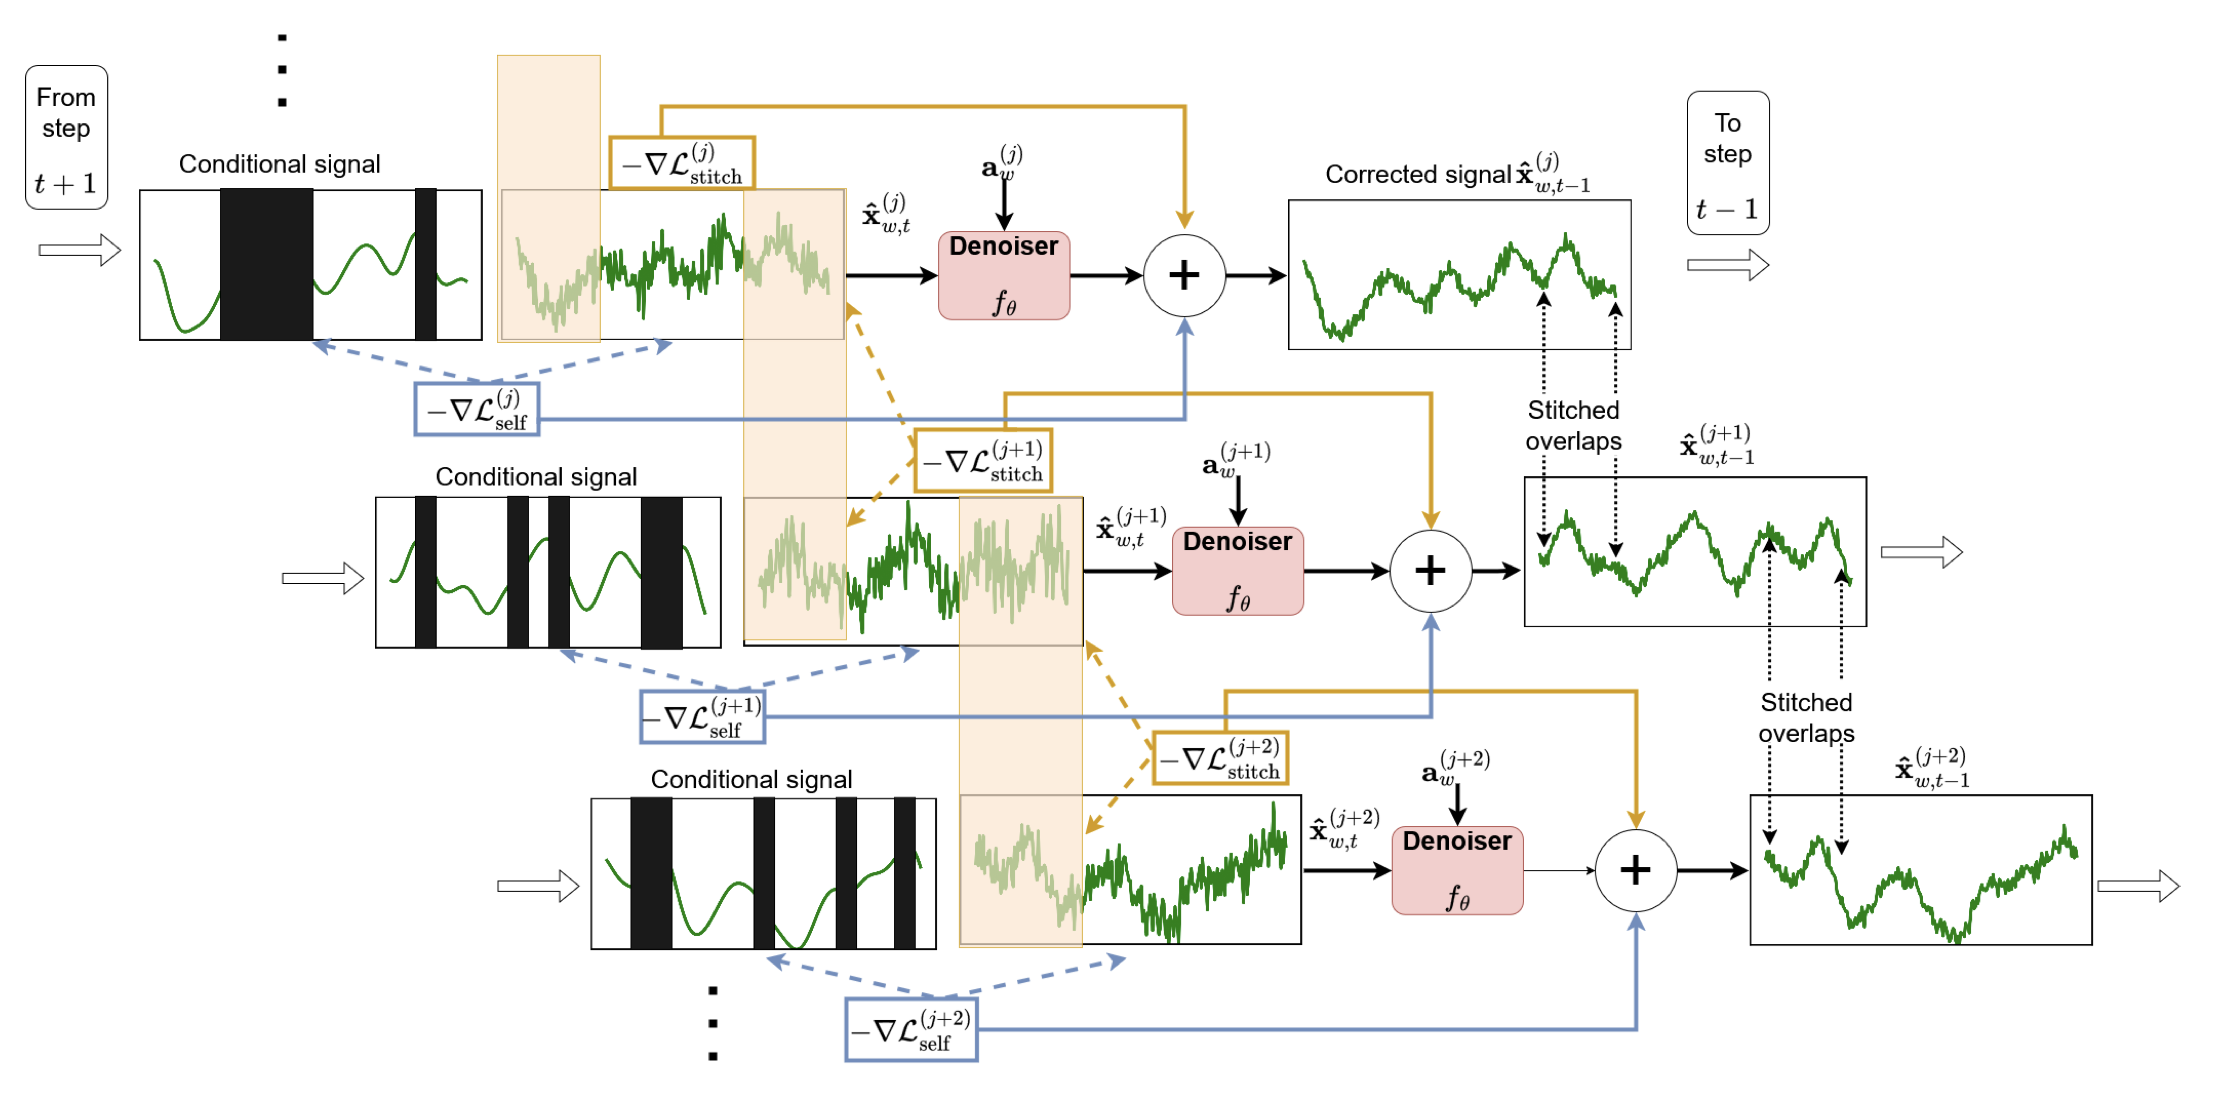
\includegraphics[width=\textwidth]{images/stitchComplex.png}
    \caption{\emph{Stitching} mechanism in WaveStitch: overlapping windows are denoised in parallel and reconciled in common areas to maintain sequential consistency. (Adapted from \cite{wavestitch}).}
    \label{fig:stitching_paper}
\end{figure}

\subsection{Cyclic encoding of categorical variables (Q3)}
The third innovation in WaveStitch concerns the representation of categorical features.  
Instead of using traditional \emph{one-hot encoding}, the authors propose a \textbf{cyclic encoding}:

\[
\theta_k = \frac{2\pi k}{K}, \quad
\text{with } k = 0,1,\dots,K-1
\]
\[
a_{sin}(k) = \sin(\theta_k), \quad a_{cos}(k) = \cos(\theta_k)
\]

Each categorical variable is then mapped to two coordinates $(\sin, \cos)$ on a unit circle.  
This approach has three main advantages:  
\begin{itemize}
    \item it drastically reduces dimensionality (from $K$ to 2 dimensions);  
    \item it preserves the cyclical nature of the variables (for example, December and January are close on the circumference, unlike what happens with one-hot encoding);  
    \item it decreases the sparsity of the input, making training more efficient~\cite{wavestitch}.  
\end{itemize}

\section{Experiments and results}

To validate the proposed approach, the authors of \textbf{WaveStitch} conducted a series of experiments on public datasets from different domains:  
\emph{Beijing Air Quality}, \emph{Metro Traffic Volume}, \emph{Panama Energy}, \emph{Rossman Sales}, and \emph{Australia Tourism}.  
These datasets include univariate and multivariate signals, including both continuous variables (e.g., energy consumption, traffic volume) and categorical features (e.g., year, month, district)~\cite{wavestitch}.

\subsection{Experimental setup}
\begin{itemize}
    \item \textbf{Hardware configuration:} The experiments were performed on an AMD Ryzen 9 5900 processor with 12 cores and an NVIDIA RTX 3090 GPU, demonstrating the need for substantial computing resources for training diffusion models.  

    \item \textbf{Data division:} The test sets were constructed to contain combinations of completely new auxiliary conditions, such as a year that was never present in the training set.  
    This made the evaluation more realistic and rigorous.  

    \item \textbf{Tasks evaluated:} imputation of missing values, short-term forecasting, and generation of synthetic scenarios under multi-level constraints (\emph{Root}, \emph{Intermediate}, \emph{Bottom}).  

    \item \textbf{Metrics:} The authors adopted a mix of point and structural metrics:  
    \begin{itemize}
        \item \emph{Mean Squared Error (MSE)} to quantify numerical accuracy;  
        \item \emph{Autocorrelation Difference (ACD)} to measure similarity in temporal patterns;  
        \item \emph{Cross-feature Correlations (x-Corr)} to evaluate dependencies between multivariate variables~\cite{wavestitch}.  
    \end{itemize}
\end{itemize}

\subsection{Main results}
The experimental results clearly show the advantages of WaveStitch:  
\begin{itemize}
    \item in terms of MSE, the model achieves up to \textbf{10 times better performance} than the baselines (e.g., TSDiff, TimeWeaver, TimeGAN), particularly in the \emph{Australia Tourism (B)} task;  

    \item the stitching mechanism allows for \textbf{460 times faster} generation than the traditional autoregressive approach, while maintaining comparable MSE values;  

    \item in structural metrics, WaveStitch better preserves autocorrelations and cross-correlations, demonstrating that it replicates not only point values but also deep statistical relationships in the data~\cite{wavestitch,tashiro2021csdi,zhou2023timeweaver,yoon2019timegan}.  
\end{itemize}

\subsection{Comparative table}
An excerpt of the results reported by the authors is shown in Table~\ref{tab:wave-results}, which summarizes the performance of WaveStitch compared to the most relevant baselines.  

\begin{table}[H]
\centering
\setlength{\tabcolsep}{10pt}
\renewcommand{\arraystretch}{1.15}
\begin{tabular}{| l | l | c | c | c |}
\hline
\rowcolor[HTML]{F87C58}
\textbf{Dataset / Task} & \textbf{Method} & \textbf{MSE} & \textbf{ACD} & \textbf{x-Corr} \\
\hline
AustraliaTourism (B) & TimeGAN~\cite{yoon2019timegan}    & 1.580 & 0.231 & 0.298 \\ \hline
                     & TSDiff/CSDI~\cite{tashiro2021csdi} & 1.420 & 0.185 & 0.271 \\ \hline
\rowcolor[HTML]{FDE5DC}
                     & WaveStitch~\cite{wavestitch}       & \textbf{0.153} & \textbf{0.072} & \textbf{0.101} \\ \hline
MetroTraffic (I)     & TimeWeaver~\cite{zhou2023timeweaver} & 0.864 & 0.210 & 0.322 \\ \hline
                     & TSDiff/CSDI~\cite{tashiro2021csdi}   & 0.701 & 0.175 & 0.285 \\ \hline
\rowcolor[HTML]{FDE5DC}
                     & WaveStitch~\cite{wavestitch}          & \textbf{0.312} & \textbf{0.090} & \textbf{0.133} \\ \hline
\end{tabular}
\caption{Comparison of methods: MSE (error), ACD (autocorrelation difference), x-Corr (correlation difference).  
The values show WaveStitch’s ability to reduce numerical error (MSE) and preserve statistical structures (ACD, x-Corr); values adapted from \cite{wavestitch}.}
\label{tab:wave-results}
\end{table}

\section{Connection to this work}

Perfect, now we know why the techniques introduced by WaveStitch can be directly applied to my work.  
Following the approach of the authors, who validated the model on benchmark datasets such as \emph{Metro Traffic} and \emph{Australia Tourism}, as I mentioned in the previous chapter, I chose to replicate the analysis, training, and evaluation flow by applying it to real energy data from the HPC center in Turin.  
In particular, the core of my work is the concepts of imputation, synthetic scenario generation, and conditional forecasting, which I will show how I have adapted to the context of monitoring rack consumption and electrical variables, with the aim of verifying the validity of the model in a complex and noisy environment.
% \chapter{Architettura del sistema e pianificazione}

% ---------------------------------
\section{Struttura del database HPC}

I dati energetici del centro HPC erano memorizzati in un \textbf{time series database} 
(\emph{InfluxDB}), scelto per la sua efficienza nella gestione di misure temporali 
con campionamenti regolari o irregolari.  

La struttura del database comprendeva:
\begin{itemize}
  \item \textbf{Measurements}: tabelle logiche contenenti le misurazioni, ad esempio 
  potenza trifase, energia cumulata, corrente per rack;
  \item \textbf{Tags}: metadati associati (es. identificativo rack, posizione, sensore);
  \item \textbf{Fields}: valori numerici (es. Watt, Volt, Ampere) registrati a intervalli regolari;
  \item \textbf{Timestamp}: chiave primaria che definisce la sequenza temporale delle osservazioni.
\end{itemize}

Questa organizzazione ha reso possibile interrogare e filtrare rapidamente i dati 
per finestra temporale, rack o tipo di misura.


% ---------------------------------
\section{Metriche e obiettivi di valutazione}

Per valutare la qualità dei dati sintetici e delle previsioni si sono definiti obiettivi chiari:
\begin{itemize}
  \item \textbf{Confronto con i dati reali}: verifica della somiglianza statistica e 
  strutturale rispetto alle serie originali;
  \item \textbf{Metriche puntuali}: MAE, RMSE, MAPE, sMAPE per misurare la fedeltà numerica;
  \item \textbf{Metriche normalizzate}: NRMSE, WMAPE per rendere comparabili dataset diversi;
  \item \textbf{Metriche strutturali}: ACD (Autocorrelation Difference) e xCorrDiff per 
  valutare autocorrelazioni e dipendenze multivariate.
\end{itemize}

Questi obiettivi hanno costituito la base per tutte le sperimentazioni successive.

% ---------------------------------
\section{Configurazione ambiente con Docker e InfluxDB}

La configurazione ha previsto:
\begin{itemize}
  \item \textbf{Containerizzazione}: ogni servizio (InfluxDB, client CLI, interfacce di supporto) 
  eseguito in container indipendenti;
  \item \textbf{Sicurezza}: gestione delle credenziali tramite \emph{Docker secrets};
  \item \textbf{Persistenza}: volumi montati per mantenere dati e configurazioni anche dopo 
  il riavvio dei container;
  \item \textbf{Accesso tramite API}: esposizione dei dati via REST API e client Python.
\end{itemize}

Questo ha garantito un ambiente portabile, stabile e facilmente replicabile.

% ---------------------------------
\section{Strumenti software utilizzati}

L’ambiente di lavoro si è basato su strumenti open-source:
\begin{itemize}
  \item \textbf{Python} per l’analisi e l’implementazione;
  \item \textbf{Pandas e NumPy} per la manipolazione dei dataset;
  \item \textbf{Matplotlib e Statsmodels} per l’analisi visiva e la decomposizione statistica;
  \item \textbf{PyTorch} come framework di deep learning per WaveStitch;
  \item \textbf{InfluxDB client} per il trasferimento dati;
  \item \textbf{Docker Compose} per l’orchestrazione dei container.
\end{itemize}

Questi strumenti hanno permesso di costruire un flusso end-to-end, dal dato grezzo 
alla generazione sintetica, mantenendo modularità e riusabilità.
\chapter{Implementation}

\section{Data Cleaning and Preprocessing}

As my Data Analysis professor always said, “you can't do much with a dirty, disturbed, and noisy dataset.”  
In fact, I started the implementation with a preliminary phase of \textbf{quality control, cleaning, and normalization of the data}, which is essential for clustering and training the generative model.  
All measurements exported from InfluxDB in CSV format underwent the same processing flow to ensure uniform treatment of energy signals and facilitate the identification of any anomalies or inconsistencies in the raw data~\cite{han2011data, aggarwal2015data}.

\subsection{Quality Check (QC) Audit}

As a first step, I implemented an automated \emph{audit} function, applied to each CSV file with the aim of verifying the quality of the original data and identifying possible critical issues before the actual cleaning phase.  
This control procedure, performed in batches on all measurements exported from InfluxDB, calculates a set of diagnostic statistics and temporal consistency indicators for each column, thus providing a quantitative overview of the dataset’s status.  
The main checks include:
\begin{itemize}
  \item the percentage of missing values (\emph{NaN \%});
  \item descriptive statistics such as standard deviation, minimum, maximum, and number of unique values (useful for identifying constant or nearly constant columns);
  \item analysis of time gaps between consecutive timestamps, by calculating the median interval and detecting any anomalous jumps~\cite{little2019statistical}.
\end{itemize}

To do this, I wrote the function shown in Listing~\ref{lst:auditcsv}, which automates the entire process on a single CSV file, returning both column statistics and an overall temporal consistency report.

\begin{listing}[H]
\begin{minted}[fontsize=\footnotesize,linenos,breaklines,frame=lines,bgcolor=lightgray!10]{python}
def audit_csv(path: Path):
    """
    Loads and analyzes a CSV file, returning:
    - Clean and temporally sorted DataFrame
    - Descriptive statistics per column
    - Diagnostics on temporal gaps
    """
    df = pd.read_csv(path, low_memory=False)
    df = df.loc[:, ~df.columns.str.contains(r"^Unnamed")]
    df["_time"] = pd.to_datetime(df["_time"], utc=True, errors="coerce")

    # Statistical analysis per column
    info = []
    for c in df.columns:
        if c == "_time": continue
        s = pd.to_numeric(df[c], errors="coerce")
        info.append({
            "column": c,
            "nan_%": round(s.isna().mean()*100, 2),
            "std": float(s.std(skipna=True)),
            "unique_vals": int(s.nunique(dropna=True))
        })

    # Diagnosis of time gaps
    dt = df["_time"].diff().dt.total_seconds()
    gaps = {"median_step_s": dt.median(), "big_gaps_%": (dt > 3*dt.median()).mean()*100}

    return df, pd.DataFrame(info), gaps
\end{minted}
\caption{Preliminary audit function for time series datasets.}
\label{lst:auditcsv}
\end{listing}

After validating the function on individual files, I applied it in batches to all measurements in the InfluxDB \emph{bucket}, allowing me to quickly identify the noisiest or most incomplete measurements.  
An excerpt from the control report obtained for the \emph{M2M} measurement is shown in Table~\ref{tab:qc_m2m}.

\begin{longtable}[H]{| l | c | c | c | c | c |}
\hline
\rowcolor[HTML]{F87C58}\textbf{Column} & \textbf{NaN \%} & \textbf{Std} & \textbf{Min} & \textbf{Max} & \textbf{Unique values} \\
\hline
\texttt{Phase 1 Power} & 0.3 & 5.12 & 12.5 & 67.1 & 1221 \\
\hline
\texttt{Phase 2 Power} & 0.1 & 4.87 & 11.8 & 69.3 & 1243 \\
\hline
\texttt{Phase 3 Power} & 0.0 & 6.04 & 13.1 & 72.4 & 1250 \\
\hline
\caption{Excerpt from the Quality Check report for the \emph{M2M} measurement.}
\label{tab:qc_m2m}
\end{longtable}

\subsection{Data Cleaning and Normalization}
\label{subsec:data-cleaning}

After completing the audit phase, I was able to proceed with the \textbf{data cleaning and normalization} process.  
This phase is crucial, as the quality and reliability of the data directly determine the robustness of subsequent analyses~\cite{little2019statistical, aggarwal2015data}.  
I implemented the \emph{data cleaning} flow in a systematic and reusable way, applying it to all time series exported from InfluxDB.  
The pipeline follows a sequence of operations typical of analyses, adapted to the specificities of my dataset.

\begin{listing}[H]
\begin{minted}[fontsize=\footnotesize,linenos,breaklines,frame=lines,bgcolor=lightgray!10]{python}
def clean_timeseries_df(
    df_raw: pd.DataFrame,
    min_std: float = 1e-3,
    interpolate_limit: int = 3,
    resample_rule: str | None = None,      # e.g. "5T"
    winsorize: bool = True,
    winsor_limits=(0.01, 0.99)
) -> pd.DataFrame:
    df = df_raw.copy()
    df["_time"] = pd.to_datetime(df["_time"], utc=True, errors="coerce")
    df = df.dropna(subset=["_time"]).sort_values("_time").set_index("_time")

    # removal of empty or nearly constant columns
    df = df.apply(pd.to_numeric, errors="coerce")
    df = df.dropna(axis=1, how="all")
    df = df.loc[:, df.std(skipna=True) > min_std]

    # aggregation of time duplicates
    if df.index.has_duplicates:
        df = df.groupby(level=0).mean(numeric_only=True)

    # clipping per column to quantiles (winsorization)
    if winsorize:
        q_low, q_hi = df.quantile(winsor_limits[0]), df.quantile(winsor_limits[1])
        for c in df.columns:
            if q_low[c] < q_hi[c]:
                df[c] = df[c].clip(lower=q_low[c], upper=q_hi[c])

    # interpolation and (optional) resampling
    df = df.interpolate(method="time", limit=interpolate_limit, limit_direction="both")
    if resample_rule:
        df = (df.resample(resample_rule)
                .mean(numeric_only=True)
                .interpolate(limit=interpolate_limit, limit_direction="both"))

    return df.reset_index()
\end{minted}
\caption{Dataset cleaning function: temporal parsing, removal of quasi-constant columns, winsorization, and interpolation.}
\end{listing}

First, I convert all timestamps to UTC datetime format, sorting the rows in chronological order and removing any records without a time reference.  
Next, I transform each column into numerical format, eliminating those that are completely empty or nearly constant, i.e., characterized by a negligible standard deviation or a zero minimum–maximum range.  
In the case of temporal duplicates, I consolidate the corresponding rows by calculating the average of the values, so as to obtain a monotonic and consistent time sequence.  
To mitigate the impact of outliers, I then apply \textbf{winsorization} to each column, limiting extreme values to quantiles $[q_{\ell}, q_{h}]$.  
This technique preserves the statistical structure of the central data while reducing the influence of outliers without eliminating them completely.  
For short-term gaps, I perform \emph{time-based} (linear in time) interpolation up to a maximum of three consecutive samples.  
Finally, the function offers the possibility of performing a fixed-step \textbf{resampling} (e.g., every 5 minutes), so as to standardize the sampling frequency between the different measurements and make the series more comparable~\cite{shumway2017time, box2015time}. Once the cleaning was complete, I proceeded to save the datasets in CSV format, sorting the columns deterministically (starting with \texttt{\_time}) and optimizing file size by \textbf{downcasting to} \texttt{float32}.  
This choice allowed me to significantly reduce disk space while maintaining the accuracy necessary for subsequent analyses~\cite{aggarwal2015data}.

\begin{listing}[H]
\begin{minted}[fontsize=\footnotesize,linenos,breaklines,frame=lines,bgcolor=lightgray!10]{python}
def save_clean(df_clean: pd.DataFrame, out_path: Path):
    cols = ["_time"] + sorted([c for c in df_clean.columns if c != "_time"])
    df_clean = df_clean.loc[:, cols]
    for c in df_clean.columns:
        if c != "_time":
            df_clean[c] = pd.to_numeric(df_clean[c], errors="coerce").astype("float32")
    out_path.parent.mkdir(parents=True, exist_ok=True)
    df_clean.to_csv(out_path, index=False)
    return out_path
\end{minted}
\caption{Function for saving clean datasets with stable sorting and numerical optimization.}
\end{listing}

Thanks to this process, I obtained consistent datasets, free of spurious or redundant columns and more robust with respect to the presence of outliers and time gaps.  
All the files used in the subsequent stages of \emph{exploratory analysis}, \emph{clustering}, and \emph{generative training} derive from these cleaned and normalized CSV files.

% ---------------------------

\section{Exploratory analysis and clustering}

After completing the \emph{data cleaning} phase, I began a systematic process of \textbf{exploratory data analysis} (EDA) with the aim of understanding the statistical structure of the energy variables and identifying the most informative fields to be used in the subsequent generative training phase~\cite{han2011data,bishop2006pattern,hastie2009elements}.  
The analysis started from the \emph{M2M} measurement, chosen as a representative case study as it aggregates the behavior of a complete three-phase system, and was then extended to the main selected \emph{Rack*pduA}.

\subsection{Visualization of the main variables}

To study the temporal trend of the most significant electrical signals, I selected the fields relating to current, voltage, power, and energy, generating an independent graph for each.  
This allowed me to identify long-term trends, daily cycles, and the presence of noise or local anomalies in the data~\cite{box2015time,shumway2017time}.

\begin{listing}[H]
\begin{minted}[fontsize=\footnotesize,breaklines,linenos,frame=lines,bgcolor=lightgray!10]{python}
import matplotlib.pyplot as plt

selected_fields = [
    "L1 Current", "L2 Current", "L3 Current",
    "Phase Voltage L1", "Phase Voltage L2", "Phase Voltage L3",
    "3Phase System Voltage", "Apparent Power L2",
    "3Phase System Frequency", "3Phase System Current",
    "3Phase System Apparent Power", "3Phase System Active Power AVG",
    "3Phase System Active Power", "3Phase System Active Energy"
]

df_sel = df_m[["_time"] + selected_fields].copy()

fig, axs = plt.subplots(len(selected_fields), 1, figsize=(15, 3 * len(selected_fields)))
for i, col in enumerate(selected_fields):
    axs[i].plot(df_sel["_time"], df_sel[col], label=col)
    axs[i].set_title(col); axs[i].set_xlabel("Time"); axs[i].grid(True)
plt.tight_layout(); plt.show()
\end{minted}
\caption{Temporal display of the main electrical variables of the measurement \texttt{M2M}.}
\end{listing}

From inspecting the graphs, I observed a clear cyclical behavior in active and apparent power, consistent with typical HPC system loads. Phase voltages, on the other hand, showed greater local variability, indicating instrumental noise or fluctuations in the power supply network.

\subsection{Correlation between variables}

To quantify the linear relationships between the energy fields, I calculated \textbf{Pearson's correlation matrix} on the main signals of the \emph{M2M} measurement, then extended the same procedure to the other measurements.  
The resulting heat map highlights:
\begin{itemize}
  \item strong correlations between \emph{phase currents} and \emph{active powers} ($r \approx 0.9$–$0.95$);
  \item almost perfect correlations between \emph{phase voltages} ($r \approx 0.99$);
  \item a very weak correlation between the \emph{system frequency} and the other quantities;
  \item a moderate correlation between \emph{active energy} and power, consistent with its cumulative behavior.
\end{itemize}

\begin{listing}[H]
\begin{minted}[fontsize=\footnotesize,breaklines,linenos,frame=lines,bgcolor=lightgray!10]{python}
import seaborn as sns

# Only numeric columns (excluding timestamp)
corr = df_selected.drop(columns="_time").corr()
plt.figure(figsize=(10, 8))
sns.heatmap(corr, annot=True, fmt=".2f", cmap="coolwarm", square=True)
plt.title(f"Correlation between field - {measurement}")
plt.tight_layout()
plt.show()
\end{minted}
\end{listing}

\begin{figure}[H]
\centering
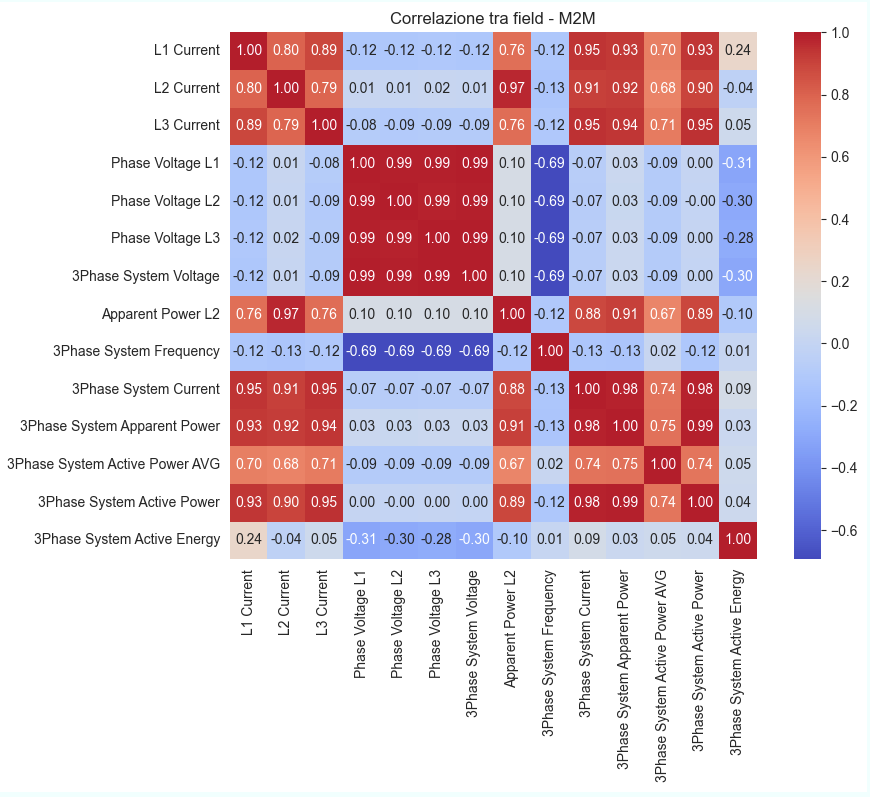
\includegraphics[width=0.85\textwidth]{images/matr_corr.png}
\caption{Correlation matrix between the main electric fields of the \emph{M2M} measurement.}
\label{fig:m2m_heatmap}
\end{figure}

This analysis allowed me to identify groups of highly correlated and redundant variables, providing a solid basis for the subsequent selection of the most representative features to be used in clustering and generation models~\cite{bishop2006pattern,han2011data,hastie2009elements,pearson1895correlation}.

\subsection{Autocorrelation of signals}

I deepened the temporal analysis by focusing on the variable \texttt{3Phase System Active Power AVG}, which summarizes the overall energy behavior of the system.  
I calculated the \textbf{autocorrelation function} (\emph{ACF}) up to 100 delays, highlighting a slow decay and the presence of \textbf{cyclical patterns} attributable to daily and weekly periodicity.

\begin{listing}[H]
\begin{minted}[fontsize=\footnotesize,breaklines,linenos,frame=lines,bgcolor=lightgray!10]{python}
from statsmodels.graphics.tsaplots import plot_acf

plot_acf(df_selected["3Phase System Active Power AVG"].dropna(), lags=100)
plt.title("Autocorrelation - 3Phase System Active Power AVG")
plt.show()
\end{minted}
\end{listing}

\begin{figure}[H]
\centering
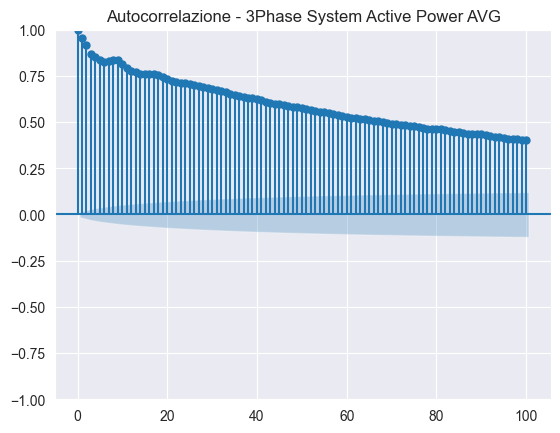
\includegraphics[width=0.7\textwidth]{images/autocorrelation_m2m.png}
\caption{Autocorrelation function (\emph{ACF}) of the average three-phase power (\emph{M2M}) up to 100 delays.}
\label{fig:m2m_autocorr}
\end{figure}

The ACF analysis provided two key insights:
\begin{enumerate}
  \item energy loads in HPC systems are not purely random, but follow regular cycles linked to the use of computational resources~\cite{box2015time,shumway2017time};
  \item the presence of stable periodicity justifies the introduction of \textbf{cyclic features} (sine and cosine of hour, day, and month) in the preprocessing pipeline, making the intrinsic seasonality of the data explicit and improving the model's ability to learn recurring patterns~\cite{bishop2006pattern,hastie2009elements}.
\end{enumerate}

\subsection{Clustering with PCA and \textit{k}-Means}

To identify \textbf{latent structures} within energy signals from HPC systems, I developed a multi-step clustering workflow that integrates statistical analysis, dimensionality reduction, and visual interpretation of data.  
The objective of this phase was twofold: on the one hand, I needed to understand the intrinsic variability of the signals and identify recurring operating regimes; on the other hand, I needed to provide a compact and interpretable representation of the data for the subsequent phases~\cite{bishop2006pattern,hastie2009elements,han2011data,aggarwal2015data}.

\begin{enumerate}
  \item \textbf{Feature extraction.}  
  I divided each signal into time windows of 128 steps (with stride 64) and calculated a set of statistical and dynamic descriptors for each window—mean, standard deviation, RMS energy, mean slope, and lag-1 autocorrelation—for each power channel.  
  This approach allowed me to transform the continuous time series into a structured set of numerical vectors, more suitable for multivariate analysis.

  \item \textbf{Cleaning and scaling.}  
  I subjected the features obtained in this way to a robust normalization process to ensure greater numerical stability and reduce the influence of outliers or annoying measurement noise.  
  In particular, I performed:
  \begin{itemize}
      \item removal of constant or entirely null columns;
      \item imputation of missing values with the median for each feature;
      \item \emph{clipping} at the 1st–99th percentile to attenuate outliers;
      \item the application of a \emph{RobustScaler} (based on quantiles 5–95\%) to obtain a stable and comparable distribution between features.
  \end{itemize}

\begin{listing}[H]
\begin{minted}[fontsize=\footnotesize,breaklines,linenos,frame=lines,bgcolor=lightgray!10]{python}
from sklearn.preprocessing import RobustScaler
import numpy as np

F = Feat_tr.astype("float64")
F[~np.isfinite(F)] = np.nan
col_med = np.nanmedian(F, axis=0)
inds = np.where(np.isnan(F))
if inds[0].size: F[inds] = np.take(col_med, inds[1])
var = np.var(F, axis=0)
F = F[:, var > 1e-12]                # removes quasi-constants
lo, hi = np.quantile(F, [0.01, 0.99], axis=0)
F = np.clip(F, lo, hi)               # clipping outliers
Fz = RobustScaler().fit_transform(F) # robust scaling
\end{minted}
\end{listing}

  \item \textbf{Dimensional reduction (PCA).}  
  To analyze the internal structure of the features, I applied \emph{Principal Component Analysis} (PCA), reducing the variable space to:
  \begin{itemize}
      \item 2 principal components for graphical visualization (\emph{PCA-2D});
      \item up to 10 components for the actual input to clustering (\emph{PCA-10D}).
  \end{itemize}
  This transformation allowed me to capture over 80\% of the total variance, thus preserving essential information at a reduced computational cost~\cite{jolliffe2002pca}.

  \item \textbf{k-Means and optimal selection of $k$.}  
  I then applied the \emph{k-Means} algorithm for values of $k$ between 2 and 6, evaluating the quality of each configuration using the \emph{silhouette score}, a measure of internal cohesion and separation between clusters~\cite{rousseeuw1987silhouettes}.
\end{enumerate}

\subsubsection{Evaluation and results}

Analysis of the \emph{silhouette score} values (Figure~\ref{fig:silhouette}) showed a maximum for $k=5$ ($s \approx 0.42$), indicating a clear separation between the groups and a well-defined latent structure in the data.  
The two-dimensional projections obtained with PCA show distinct and consistent clusters, interpretable as different \textbf{operating regimes} of the HPC system and its power supply subsystem.

\begin{figure}[H]
\centering
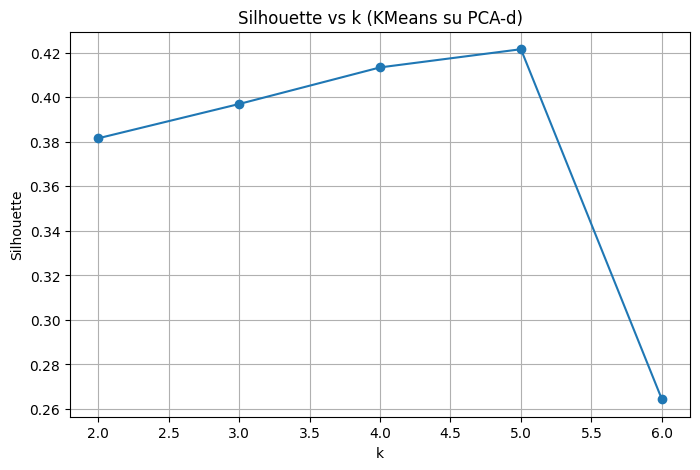
\includegraphics[width=0.50\textwidth]{images/silhouette_plot.png}
\caption{\emph{Silhouette score} trend as $k$ varies.}
\label{fig:silhouette}
\end{figure}

\begin{figure}[H]
\centering
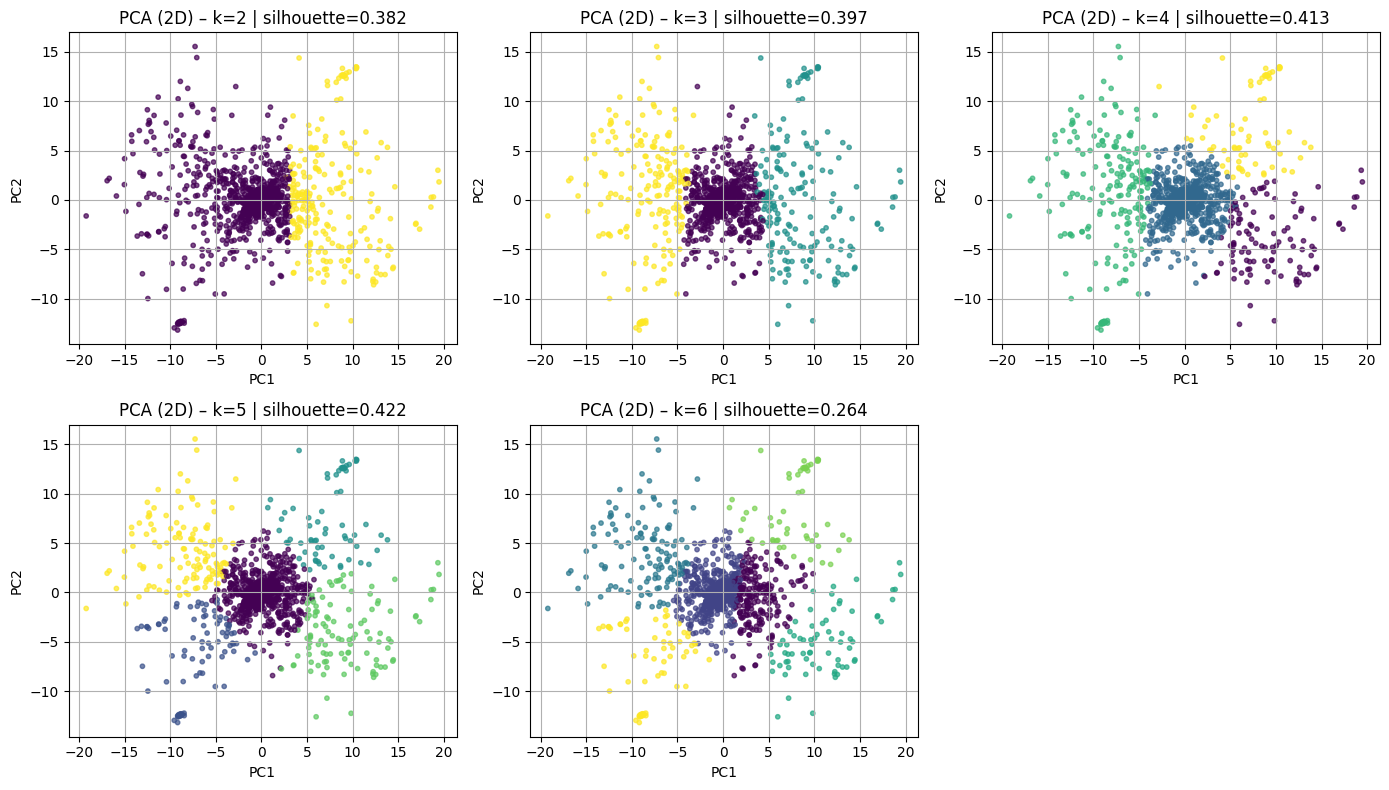
\includegraphics[width=0.70\textwidth]{images/pca2d_all_k.png}
\caption{PCA-2D projections of clusters obtained with $k = 2 \dots 6$.  
A progressive refinement of the separation can be observed up to $k=5$, beyond which the clusters begin to fragment.}
\label{fig:pca2d_all_k}
\end{figure}

\begin{figure}[H]
\centering
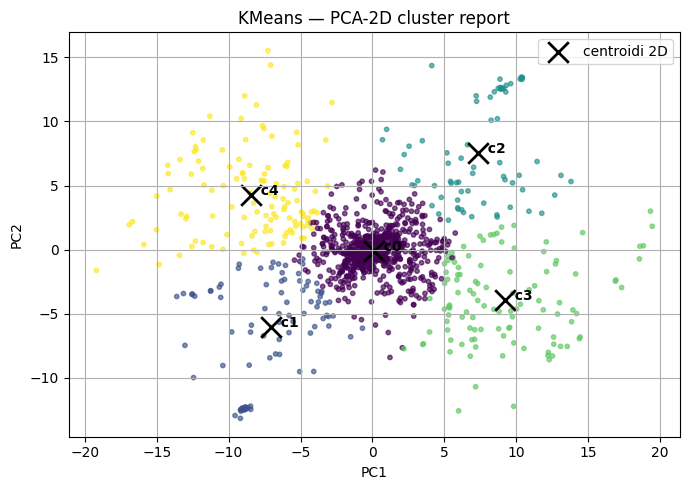
\includegraphics[width=0.50\textwidth]{images/pca2d_cluster_report.png}
\caption{Distribution of data in PCA-2D space with labeled centroids for each cluster ($k=5$).  
There is a clear separation between the density regions, corresponding to different energy regimes.}
\label{fig:pca2d_cluster_report}
\end{figure}

\subsubsection{Interpretation of clusters}

As I mentioned, analysis of the results allowed me to identify three main categories of behavior:
\begin{itemize}
  \item \textbf{Stable clusters}, characterized by almost constant signals and associated with basic loads or periods of system inactivity;
  \item \textbf{Dynamic clusters}, with rapid variations and power peaks, typical of periods of intense computing;
  \item \textbf{Intermediate clusters}, interpretable as transitional states or partial activity between the two extremes.
\end{itemize}

These partitions provide a clear representation of \textbf{recurring energy patterns} in the racks and form an empirical basis for the subsequent \textbf{conditional generation of synthetic series} using diffusion models such as \emph{WaveStitch}.

% ----------------------

\section{Training, scenario imputation, and conditional generation with WaveStitch}

After completing the steps described so far, I finally started the \textbf{training and conditional generation} phase with the \emph{WaveStitch} model.  
This part of the work represents the experimental core of my project, with the interesting aim of: on the one hand, evaluating the model's ability to adapt to real data affected by noise and irregularities; on the other hand, verifying the possibility of producing \textbf{plausible synthetic scenarios}, useful for simulation, testing, and much more.

\subsection{Model training}

I began training with the \emph{M2M} metric, selected for its regularity and its ability to represent, as I mentioned earlier, the overall energy performance of the HPC system.  
The configuration adopted for training was defined in order to balance complexity, stability, and generalization capacity, with the following main hyperparameters:

\begin{itemize}
  \item \textbf{Backbone}: \texttt{S4}, chosen for its efficiency in modeling long sequences using structured memory;
  \item \textbf{Window size}: 96, to capture a broader and more informative temporal context;
  \item \textbf{Stride}: 8, to ensure high overlap and improve continuity between successive windows;
  \item \textbf{Epochs}: 100, ensuring stable convergence of the learning process;
  \item \textbf{Batch size}: 64, balancing numerical stability and memory limitations;
  \item \textbf{Diffusion timesteps}: 200, higher than those in the original paper to handle the greater variability of HPC signals;
  \item \textbf{Cyclic features}: \texttt{month, day, hour}, useful for capturing daily and seasonal periodicity.
\end{itemize}

To ensure flexibility in experimentation, I created a parametric Python script that dynamically constructs the execution command of the \texttt{training\_wavestitch.py} file, allowing training sessions to be started in a controlled manner on different datasets and with variable configurations~\cite{gu2021s4}.

\begin{listing}[H]
\begin{minted}[fontsize=\footnotesize,breaklines,linenos,frame=lines,bgcolor=lightgray!10]{python}
cmd = [
    sys.executable, "training_wavestitch.py",
    "-dataset", DATASET,
    "-backbone", BACKBONE,
    "-window_size", str(WINDOW_SNE),
    "-stride", str(STRIDE),
    "-epochs", str(EPOCHS),
    "-batch_size", str(BATCH_SNE),
    "-hdim", str(HDIM),
    "-layers", str(LAYERS),
    "-timesteps", str(TIMESTEPS),
    "-s4_dropout", str(S4_DROPOUT),
    "-propCycEnc", PROP_CYC,
]
res = subprocess.run(cmd, text=True, capture_output=True)
print(res.stdout)
\end{minted}
\end{listing}

The resulting model is saved in an \textbf{enriched checkpoint}, which not only contains the weights of the neural network, but also includes: the complete configuration of the training hyperparameters, the ordered list of the dataset columns, the indication of cyclic and non-cyclic features, and the actual input and output dimensions.  
The final checkpoint was named \texttt{model\_prop.pth}, indicating the presence of cyclic features (\emph{propCycEnc}) in the training.

\begin{figure}[H]
\centering
\begin{tikzpicture}[
    font=\footnotesize\sffamily,
    node distance=1.8cm,
    process/.style={
        rectangle, rounded corners,
        draw=black, very thick,
        text centered,
        minimum width=4.2cm,
        minimum height=1.1cm,
        align=center
    },
    arrow/.style={thick,->,>=stealth}
]
\node[process, fill=cyan!15] (prep) {Preprocessing\\\textit{(scaling, encoding)}};
\node[process, fill=teal!15,  below=of prep] (win) {Windowing\\\textit{(windowing, stride)}};
\node[process, fill=lime!15,  below=of win]  (train) {Training\\\textit{(denoising)}};
\node[process, fill=gray!15,  below=of train] (ckpt) {Checkpoint\\\textit{rich (.pth)}};

\draw[arrow] (prep) -- (win);
\draw[arrow] (win)  -- (train);
\draw[arrow] (train) -- (ckpt);

\node[right=0.7cm of prep]  {\texttt{df\_cleaned}};
\node[right=0.7cm of win]   {\textit{window size = 96, stride = 8}};
\node[right=0.7cm of train] {\textit{loss MSE, 100 epochs}};
\node[right=0.7cm of ckpt]  {\texttt{model\_prop.pth}};
\end{tikzpicture}
\caption{Simplified diagram of the training phase: preprocessing $\rightarrow$ windowing $\rightarrow$ denoising $\rightarrow$ rich checkpoint.}
\label{fig:training_pipeline}
\end{figure}

This configuration produced \textbf{stable convergence} on the \emph{M2M} data, with a progressive reduction in loss and final values comparable to those reported in the original work~\cite{wavestitch,ho2020ddpm,dhariwal2021improved}.  
Doing the same with the racks, I can say that the result demonstrated how effectively \emph{WaveStitch} can adapt to real datasets, which are noisier and more complex than the original benchmarks, confirming its robustness and generalization capabilities.

\subsection{Conditional synthetic generation}

After completing the training phase, I started the \textbf{conditional synthetic generation} using the previously trained \emph{rich checkpoint}, without the need for retraining.  
The procedure was managed using the script:\\
\texttt{synthesis\_wavestitch\_pipeline\_strided\_preconditioning.py},  
which automatically reads the hyperparameters from the checkpoint and realigns all key parameters — \emph{backbone}, window, stride, and number of \texttt{timesteps} — ensuring perfect consistency between the training and generation phases~\cite{wavestitch,ho2020ddpm,dhariwal2021improved}.  
To explore different temporal granularities of imputation, I defined three distinct scenarios: \textbf{F (Fine)} — point imputation, suitable for local \emph{forecasting}; \textbf{C (Coarse)} — reconstruction of extended time blocks or those with significant gaps; \textbf{M (Mid)} — intermediate scenario, useful for modeling transitions or progressive variations.

In order to improve the multivariate fidelity and temporal continuity of the generated sequences, I introduced two fundamental extensions: a \textbf{configurable stitching loss} in the overlap areas between parallel windows, based on \texttt{mse}, \texttt{mae}, or shape-based metrics (\texttt{cosine}, \texttt{pearson})~\cite{dhariwal2021improved,ho2020ddpm}; a \textbf{correlation regularization between channels} (\(\lambda_{\text{corr}} = 0.30\), \texttt{pearson} metric), to preserve the statistical relationships between connected variables such as currents and powers~\cite{bishop2006pattern,hastie2009elements}.


\begin{listing}[H]
\begin{minted}[fontsize=\footnotesize,breaklines,linenos,frame=lines,bgcolor=lightgray!10]{python}
# Synthesis consistent with checkpoint, three masks: F / C / M
for mask in MASKS:
    out_dir_mask = os.path.join(BASE_OUT, mask)
    os.makedirs(out_dir_mask, exist_ok=True)

    cmd = [
        sys.executable, SYNTH_SCRIPT,
        "-dataset", DATASET,
        "-backbone", BACKBONE,
        "-window_size", str(WINDOW_SIZE),
        "-stride", str(STRIDE),
        "-timesteps", str(TIMESTEPS),
        "-hdim", str(HDIM),
        "-layers", str(LAYERS),
        "-batch_size", str(BATCH_SIZE_SYNTH),
        "-synth_mask", mask,
        "-n_trials", "1",
        "-propCycEnc", PROP_CYC,
        "-s4_lmax", str(S4_LMAX),
        "-s4_dstate", str(S4_DSTATE),
        "-s4_dropout", str(S4_DROPOUT),
        "-s4_layernorm", str(S4_LAYERNORM),
        "-ckpt", CKPT,
        "-lambda_corr", str(LAMBDA_CORR),
        "-corr_mode", CORR_MODE,
        "-out_dir", out_dir_mask,
    ]

    print("[CMD] " + " ".join(shlex.quote(c) for c in cmd))
    res = subprocess.run(cmd, text=True, capture_output=True)
# (repeat with -synth_mask C and M)
\end{minted}
\caption{Conditional synthesis pipeline with automatic checkpoint alignment and multiscenario generation.}
\end{listing}

Each run generates two separate files: \texttt{real.csv}, containing the actual reference segment, and \texttt{synth*.csv}, representing the synthetic output produced by the model.

\subsection{Preliminary observations}

The first experiments conducted on my datasets showed that \emph{WaveStitch}, even in the presence of noise and outliers, is able to generate sequences \textbf{that are statistically consistent} with the overall properties of the real data.  
Looking at the point-by-point comparison, I noticed that the synthetic data tends to smooth out the most extreme peaks, producing more regular and realistic curves.  
This behavior, while reducing the local linear correlation with the original series, actually confirms the model’s remarkable ability to \textbf{generalize plausible behaviors} instead of rigidly replicating the outliers present in the source data.  

Throughout this process, I was able to observe the excellent \textbf{computational scalability} of the model.  
Thanks to the \emph{parallel generation mechanism with stitching}, the synthesis proved to be very fast, in line with the results of the original work.  
The ability to dynamically adjust the \emph{stitching} and \emph{correlation regularization} components made the pipeline flexible and adaptable to multiple experimental scenarios, ranging from short-term \emph{forecasting} to the imputation of missing time blocks.

\subsection{Extension to other HPC datasets}

As I mentioned, I replicated the entire training and synthesis process on individual rack measurements, which are characterized by greater noise and temporal irregularities.  
This systematic comparison between aggregated and local datasets allowed me to confirm that \textbf{the quality and regularity of the input signal directly influence the stability and statistical fidelity of the synthetic generation}.  
The quantitative results (MAE, RMSE, MAPE, Pearson correlation) and qualitative analyses (visual analysis, autocorrelations, and cross-correlations) will be explored in more detail in the following chapters, where I will show how \emph{WaveStitch} consistently reproduces both the average trends and the temporal structure of HPC energy signals.
% -----------------------------

\subsection{Imputation of missing values with WaveStitch}

The most valuable part of my work consists of the following three phases.  
I started by imputing missing values, which represented the most direct test of \textbf{conditional generation} based on \emph{WaveStitch}.  
The goal is to estimate the missing values $y^{\star}(t)$ at unobserved times $\mathcal{M}$, starting from a real series $y(t)$ and the synthetic trajectory $\tilde{y}(t)$ produced by the model~\cite{box2015time,shumway2017time}:
\[
y^{\star}(t) \approx \tilde{y}(t) \quad \text{for } t \in \mathcal{M}.
\]

In the event that the \texttt{real.csv} file does not contain null values, I introduced an artificial mask with amplitude $|\mathcal{M}| = 100$, so that I could quantitatively evaluate the quality of the imputation with respect to the original \emph{ground truth}~\cite{little2019statistical}.  
In this way, I was able to accurately quantify the effectiveness of the model even in the absence of truly missing data.

\begin{figure}[H]
\centering
\begin{tikzpicture}[
    every node/.style={font=\small},
    real/.style={draw, very thick, fill=gray!25, minimum height=0.55cm, minimum width=0.55cm},
    nan/.style={draw, very thick, fill=white, dashed, minimum height=0.55cm, minimum width=0.55cm},
    imputed/.style={draw, very thick, fill=blue!30, minimum height=0.55cm, minimum width=0.55cm}
]
\def\N{9}\def\xStart{0.8}\def\dx{0.95}\def\yReal{0.8}\def\yImpu{-0.2}
\def\nanA{4}\def\nanB{6}

\node[anchor=east] at (0.2,\yReal) {\textbf{Real series (with NaN)}};
\node[anchor=east] at (0.2,\yImpu) {\textbf{Imputed series (post WaveStitch)}};

\foreach \k in {0,...,\numexpr\N-1\relax} {
  \pgfmathsetmacro\x{\xStart + \k*\dx}
  \ifnum\k=\nanA \node[nan] at (\x,\yReal) {}; 
  \else\ifnum\k=\nanB \node[nan] at (\x,\yReal) {}; 
  \else \node[real] at (\x,\yReal) {}; 
  \fi\fi
  
  \ifnum\k=\nanA \node[imputed] at (\x,\yImpu) {}; 
  \else\ifnum\k=\nanB \node[imputed] at (\x,\yImpu) {}; 
  \else \node[real] at (\x,\yImpu) {}; 
  \fi\fi
}

\pgfmathsetmacro{\xa}{\xStart + \nanA*\dx}
\pgfmathsetmacro{\xb}{\xStart + \nanB*\dx}
\draw[->, thick, blue!60!black] (\xa,\yReal-0.27) -- (\xa,\yImpu+0.27);
\draw[->, thick, blue!60!black] (\xb,\yReal-0.27) -- (\xb,\yImpu+0.27);

\end{tikzpicture}
\caption{Conceptual diagram of imputation: NaNs (white, dashed) are replaced by imputed values (blue) generated by WaveStitch.}
\label{fig:imputation_schema}
\end{figure}

\paragraph{Alignment and selection of the target column.}
Since the \texttt{real.csv} and \texttt{synth*.csv} files may have slightly misaligned timestamps, I implemented a \textbf{merge-as-of} alignment, based on a nearest-neighbor match on times~\cite{han2011data}.  
This choice ensures robustness even in the presence of minimal sampling differences.  
The column of interest $v$ is identified through a hierarchical selection procedure:  
if the user provides an explicit \texttt{value\_col} parameter, I use that;  
otherwise, the function automatically attempts to detect common columns (e.g., \texttt{3Phase System Active Power AVG});  
as a last fallback, it chooses the first numeric column shared between real and synthetic files — avoiding common mistakes such as accidentally selecting the timestamp column as the target variable.

\paragraph{Affine calibration and clipping.}
To compensate for possible differences in scale or offset between real and synthetic data, I introduced an \textbf{affine calibration}:
\[
\hat{y}_{\text{synth}}(t) = a \cdot y_{\text{synth}}(t) + b,
\]
with $(a,b)$ estimated via linear regression on the observed points $t \in \mathcal{O}$~\cite{han2011data}.  
I considered two operating modes:
\begin{itemize}
  \item \textbf{Global}, which estimates $(a,b)$ across the entire series — more stable but less sensitive to regime changes;
  \item \textbf{Local}, which estimates $(a_\ell,b_\ell)$ for each contiguous block of NaN within a window $\pm W$, more suitable for non-stationary or drifting signals.
\end{itemize}

Finally, I applied a \textbf{quantile clipping} on $[q_\ell,q_h] = [0.01,0.99]$, anchoring the scale to the real signal support and reducing the impact of outliers and heavy tails~\cite{little2019statistical,aggarwal2015data}.

\paragraph{Filling strategy.}
The imputation process consists of four steps:
\begin{enumerate}
  \item optional generation of artificial NaNs (for quantitative evaluation);
  \item estimation of affine parameters $(a,b)$ or $(a_\ell,b_\ell)$ on observed points only;
  \item reconstruction of missing values through affine transformation:
  \[
  y^\star(t) =
  \begin{cases}
  a_\ell\,y_{\text{synth}}(t)+b_\ell, & \text{if \texttt{calibrate=local}}, \\[2pt]
  a\,y_{\text{synth}}(t)+b, & \text{otherwise;}
  \end{cases}
  \]
  \item \emph{tapering at the edges}, i.e., a linear blending on $\pm$ \texttt{half\_window} to eliminate discontinuities at the hole boundaries~\cite{shumway2017time}.
\end{enumerate}

\paragraph{Control parameters and robustness.}
I clearly designed the function to be adaptable to different inputs and distinct datasets.  
Thanks to this configuration, the function proved to be robust on heterogeneous data, able to automatically handle differences in sampling, scaling, and naming without manual intervention.

\begin{listing}[H]
\begin{minted}[fontsize=\footnotesize,breaklines,linenos,frame=lines,bgcolor=lightgray!10]{python}
# WaveStitch-guided imputation with calibration and clipping
csv_path, metrics = impute_missing_with_wavestitch(
    dataset="M2M", mask="M",
    base_path="notebooks/generated",
    value_col=None,          # automatic selection of target column
    n_missing=100,           # artificial mask for quantitative evaluation
    calibrate="local",       # calibration for NaN blocks
    local_window=100,        # window width ±W
    clip_quantiles=(0.01,0.99)  # clipping for energy outliers
)
print(metrics)  # -> MAE / RMSE / Corr on masked positions
\end{minted}
\caption{Example of imputation with WaveStitch and quantitative evaluation.}
\label{lst:wavestitch_imputation}
\end{listing}

I achieved an excellent compromise between fidelity and numerical stability simply by combining \texttt{calibrate=local} and \texttt{clip\_quantiles=(0.01,0.99)}, maintaining consistency even on noisy signals or those affected by outliers~\cite{little2019statistical,shumway2017time}.

\paragraph{Empirical observations.}
In tests conducted on \emph{M2M} (mask M), the \textbf{global calibration} produced regular and conservative estimates, while the \textbf{local calibration} significantly improved the reconstruction of long gaps and transitions between different regimes.  
The \textbf{clipping} reduced the effect of extreme values, improving the MAE and RMSE metrics, while the \textbf{tapering} eliminated visual discontinuities at the edges of the imputed segments.  
Overall, the results show a solid balance between statistical fidelity and signal regularity, with average correlation values $r > 0.9$ on artificial masks, as I will show in the next chapter.

% -------------------------

\subsection{Simulation of scenarios via STL decomposition}

To explore hypothetical \emph{what--if} scenarios on the energy consumption profiles of HPC systems, I implemented a simulation procedure based on the \textbf{STL seasonal decomposition} (\emph{Seasonal-Trend decomposition using Loess}).  
The goal was to understand how the different components—trend, seasonality, and residual—contribute to the overall shape of the signals, and how their modulation could simulate operational variations, drifts, or local shocks.  
Formally, the real series $y(t)$ is decomposed into three main components:
\[
y(t) = T(t) + S(t) + R(t),
\]
where $T(t)$ represents the long-term trend, $S(t)$ the seasonal cyclic component, and $R(t)$ the unstructured residual.  
Starting from this decomposition, I introduced three scaling factors $(\alpha, \beta, \gamma)$ and a local shock term $\Delta$ to construct new synthetic scenarios:
\[
y_{\text{scen}}(t) = \beta \, T(t) + \alpha \, S(t) + \gamma \, R(t) + \mathbf{1}_{\{t=t^\star\}} \cdot \Delta.
\]
This formulation makes it possible to amplify or attenuate seasonality, modify long-term trends, control residual noise, and introduce controlled impulse peaks—for example, to simulate sudden load events or temporary failures.

\paragraph{Conceptual diagram.}
\begin{figure}[H]
\centering

\begin{tikzpicture}[
    every node/.style={font=\small},
    rect/.style={draw, very thick, minimum width=0.6cm, minimum height=0.5cm},
    arrow/.style={thick,->,>=stealth}
]
% Real series
\node[anchor=east] at (-0.5,1.0) {\textbf{Real series}};
\foreach \x in {0,1,...,7}{
    \node[rect, fill=gray!25] (r\x) at (\x,1) {};
}
\node[rect, fill=white] (r3) at (3,1) {};
\node[rect, fill=white] (r4) at (4,1) {};

% STL scenario
\node[anchor=east] at (-0.5,-0.6) {\textbf{STL scenario}};
\foreach \x in {0,1,...,7}{
    \node[rect, fill=gray!25] (s\x) at (\x,-0.6) {};
}
\node[rect, fill=blue!20] (s3) at (3,-0.6) {};
\node[rect, fill=blue!20] (s4) at (4,-0.6) {};

% Arrows
\draw[->, thick, blue!70] (r3.south) -- (s3.north);
\draw[->, thick, blue!70] (r4.south) -- (s4.north);
\end{tikzpicture}
\caption{Conceptual diagram of STL simulation: modified values (white) are replaced with generated values (blue) after seasonal adjustment or the introduction of a local shock~\cite{shumway2017time, cleveland1990stl}.}
\label{fig:stl_schema_concettuale}
\end{figure}

\paragraph{Automatic column detection.}
Since the generated CSV files may contain heterogeneous structures, I made the \texttt{simulate\_scenario\_stl\_flex} function fully autonomous in identifying key columns.  
In particular, the function automatically detects:
\begin{enumerate}
  \item the time column, through a heuristic search among common names (\texttt{date}, \texttt{time}, \texttt{timestamp});
  \item the target value column, chosen from a list of known names or, if none are found, the first valid numeric column.
\end{enumerate}

\paragraph{Determination of the seasonal period.}
The quality of the STL decomposition depends strongly on the correct estimation of the period $P$, i.e., the number of samples that constitute a complete cycle.  
To determine $P$, I developed a robust inference strategy based on timestamps: estimating the median interval $\Delta t$ between two observations and setting
\[
P \approx \left\lfloor \frac{86400}{\Delta t} \right\rfloor,
\]
which corresponds to the average number of daily samples (e.g., $P \approx 288$ for 5-minute data, or $P \approx 24$ for hourly data).  
When the series is too short to observe multiple complete cycles, the period is reduced to $\max(2, \lfloor |y|/3 \rfloor)$ to ensure numerical stability.  
Nevertheless, I left the option to manually specify $P$ in case of prior knowledge.

\paragraph{Implementation and main parameters.}
The simulation function accepts flexible parameters to modulate the three components:
\begin{itemize}
  \item \texttt{season\_scale} $(\alpha)$ — scale of the seasonal component $S(t)$ (default 1.2);
  \item \texttt{trend\_scale} $(\beta)$ — trend amplification factor for $T(t)$ (default 1.0);
  \item \texttt{resid\_scale} $(\gamma)$ — control for residual noise $R(t)$ (default 1.0);
  \item \texttt{shock\_idx}, \texttt{shock\_mag} — time index and amplitude of a possible impulsive shock $\Delta$;
  \item \texttt{period} — STL period, calculated automatically or defined by the user.
\end{itemize}
The result is a CSV file with an additional column \texttt{\{value\_col\}\_scenario} and a preview graph showing the first 600 samples.

\paragraph{Application to the \texttt{M2M} dataset.}
I applied this procedure to the \texttt{M2M} dataset (5-minute sampling, $P = 288$) considering two scenario configurations:
\begin{enumerate}
  \item 20\% amplification of the seasonal component without shock;
  \item 30\% amplification of the seasonal component with the addition of a local shock.
\end{enumerate}

\begin{listing}[H]
\begin{minted}[fontsize=\footnotesize,breaklines,linenos,frame=lines,bgcolor=lightgray!10]{python}
# STL scenario simulation on M2M
base = "notebooks/generated"

csv_out, png_out = simulate_scenario_stl_flex(
    dataset="M2M", mask="M", base_path=base,
    value_col="3Phase System Active Power AVG",
    season_scale=1.2, trend_scale=1.0, resid_scale=1.0,
    period=288, shock_idx=None, shock_mag=0.0
)

# Variant with amplified seasonality and local shock
csv_out2, png_out2 = simulate_scenario_stl_flex(
    dataset="M2M", mask="M", base_path=base,
    value_col="3Phase System Active Power AVG",
    season_scale=1.3, trend_scale=1.0, resid_scale=1.0,
    period=288, shock_idx=10000, shock_mag=500.0
)
\end{minted}
\caption{Running the STL simulation on \texttt{M2M}: seasonal amplification and optional shock.}
\label{lst:scenario_stl_launch}
\end{listing}

Both scenarios keep $T(t)$ and $R(t)$ unchanged, allowing the impact of the periodic component alone to be isolated and analyzed.  
The progressive increase of $\alpha$ accentuates daily cyclicality without distorting the underlying trend.  
The scenario with 30\% amplified seasonality shows more reactive behavior to daily peaks, which is useful for testing the robustness of forecasting models and overall energy stability~\cite{box2015time,shumway2017time, cleveland1990stl}.

\paragraph{Limitations and interpretation.}
The STL decomposition assumes an additive structure and quasi-stationary seasonality; in the presence of regime shifts or multiplicative effects, linear scaling may over- or underestimate the true impact~\cite{cleveland1990stl,shumway2017time}.  
In such contexts, the simulated outputs should be interpreted as \textbf{qualitative what--if analyses}, useful for stress testing and strategic planning rather than for accurate point forecasting.  
Integration with conditional generation through \emph{WaveStitch}, on the other hand, enables the creation of consistent multivariate synthetic scenarios, preserving both temporal and inter-variable dependencies observed in real data—and it has been extremely satisfying to verify this in practice.

% ------------------------

\section{Conditional forecasting with WaveStitch}
\label{sec:forecasting-wavestitch}

Here we are at the third and, for me, most interesting phase. In this section, I describe the \emph{forecasting} module that I developed following the conditional generation with \emph{WaveStitch}.  
The goal was to evaluate the model’s ability to project the local dynamics of a time series toward a short-term future horizon, maintaining consistency in both scale and shape with respect to the actual data.  
My operational idea was very straightforward: once the synthetic sequence was aligned with the real series (\texttt{real.csv} and \texttt{synth*.csv}), I extracted the tail of length $h$ (the \emph{horizon}) and used it as the predictive base for the next steps.  
To compensate for possible level or scale misalignments between real and synthetic data, I applied an \textbf{affine calibration} on the observed tail, estimating the parameters $(a,b)$ by linear regression on the common endpoints:
\[
y_{\text{real}} \approx a\,y_{\text{synth}} + b,
\quad\text{with}\quad
(a,b) = \arg\min_{a,b} \| y_{\text{tail}} - (a\,x_{\text{tail}} + b) \|_2^2,
\]
possibly including ridge regularization to handle noise or high variance.  
The final forecast is then obtained by applying the same transformation to the subsequent $h$ synthetic points~\cite{bishop2006pattern,hastie2009elements}:
\[
\widehat{y}_{t+1:t+h} = a\,y^{\text{synth}}_{t+1:t+h} + b.
\]

\begin{figure}[H]
\centering
\begin{tikzpicture}[
  every node/.style={font=\small},
  box/.style={draw, thick, minimum width=0.6cm, minimum height=0.45cm, rounded corners=2pt, fill=gray!20},
  synth/.style={draw, thick, minimum width=0.6cm, minimum height=0.45cm, rounded corners=2pt, fill=gray!10},
  forecast/.style={draw, thick, minimum width=0.6cm, minimum height=0.45cm, rounded corners=2pt, fill=green!25}
]

\def\yreal{0.9}
\def\ysynth{0.2}
\def\xmin{0.3}
\def\xstep{0.7}

\node[anchor=east] at (\xmin-0.25,\yreal) {\textbf{tail (real)}};
\node[anchor=east] at (\xmin-0.25,\ysynth) {\textbf{tail (synth)}};

\foreach \i in {0,...,7} {
  \pgfmathsetmacro\x{\xmin + \i*\xstep}
  \node[box] at (\x,\yreal) {};
  \node[synth] at (\x,\ysynth) {};
}

\pgfmathsetmacro\xa{\xmin + 4*\xstep}
\pgfmathsetmacro\xb{\xmin + 7*\xstep}
\draw[decorate, decoration={brace, amplitude=3pt}] (\xa,\yreal+0.35) -- node[above=2pt]{\footnotesize estimate \(a,b\) on the tail} (\xb,\yreal+0.35);
\draw[decorate, decoration={brace, amplitude=3pt,mirror}] (\xa,\ysynth-0.35) -- node[below=2pt]{\footnotesize \(y \approx a\,x + b\)} (\xb,\ysynth-0.35);

\pgfmathsetmacro\xendcoda{\xmin + 7*\xstep + 0.3}
\pgfmathsetmacro\xstartforecast{\xendcoda + 0.6}
\pgfmathsetmacro\xcut{(\xendcoda + \xstartforecast)/2}

\draw[dashed, thick] (\xcut,-0.2) -- (\xcut,0.5);
\node[anchor=west] at (\xcut+0.08,1.45) {\footnotesize beginning of horizon \(h\)};

\foreach \i in {0,...,7} {
  \pgfmathsetmacro\x{\xstartforecast + \i*\xstep}
  \node[forecast] at (\x,\yreal) {};
}
\end{tikzpicture}
\caption{Conceptual diagram of \emph{tail forecasting}: an affine transformation \(y \approx a\,x + b\) is estimated on the real and synthetic tail, and then applied to the subsequent \(h\) steps to obtain the calibrated forecast (green).}
\label{fig:forecast_schema}
\end{figure}

\subsection{Operational pipeline}
Here too, I designed the function to be autonomous and robust with respect to the different CSV formats produced by the generation process~\cite{han2011data}.  
The flow follows these steps:
\begin{enumerate}
  \item \textbf{I/O resolution and loading:} automatic detection of \texttt{real.csv} and \texttt{synth*.csv} files in the path \texttt{<base>/<dataset>/<mask>/}.
  \item \textbf{Time alignment:} detection of the time column, conversion to \texttt{datetime}, and alignment with \emph{merge-asof} (nearest-neighbor on timestamps).
  \item \textbf{Target column selection:} automatic identification of the variable to predict (\texttt{value\_col}), searching among common names or selecting the first numeric column.
  \item \textbf{Affine estimation on the tail:} given $n_{\text{tail}}$ points, estimate $(a,b)$ via OLS regression and compute diagnostic indicators ($R^2_{\text{tail}}$, correlation).
  \item \textbf{Forecasting:} extract the last $h$ synthetic points, apply the affine transformation, and construct future timestamps while maintaining the original sampling frequency.
  \item \textbf{Persistence and graph:} save results (\texttt{.csv}, \texttt{.png}) in \texttt{<dataset>/forecast/}, including in the title the estimated values of $a,b$ and $R^2_{\text{tail}}$.
\end{enumerate}

\paragraph{Implementation extract.}
\begin{listing}[H]
\begin{minted}[fontsize=\footnotesize,breaklines,linenos,frame=lines,bgcolor=lightgray!10]{python}
def forecast_with_wavestitch_flex(dataset, mask="F", base_path=None,
                                  value_col=None, horizon=64, calibrate=True):
    # 1) Load real and synthetic data, auto-detect time and target column
    r = pd.read_csv(...); s = pd.read_csv(...)
    t_r, t_s = _auto_time_col(r), _auto_time_col(s)
    value_col = _auto_value_col(r)
    m = pd.merge_asof(r, s, left_on=t_r, right_on=t_s, direction="nearest")

    # 2) Affine calibration on the tail
    a, b, R2 = _fit_affine(m[value_col+"_synth"][-200:], m[value_col+"_real"][-200:])

    # 3) Forward h-step forecast
    fc = a * m[value_col+"_synth"][-horizon:] + b
    out = pd.DataFrame({"forecast": fc})
    out.to_csv(".../forecast.csv", index=False)
\end{minted}
\caption{Excerpt from the forecasting function: alignment, calibration, and prediction.}
\end{listing}

\subsection{Forecast example (M2M, mask F, \texorpdfstring{$h{=}32$}{h=32})}
\begin{figure}[H]
\centering
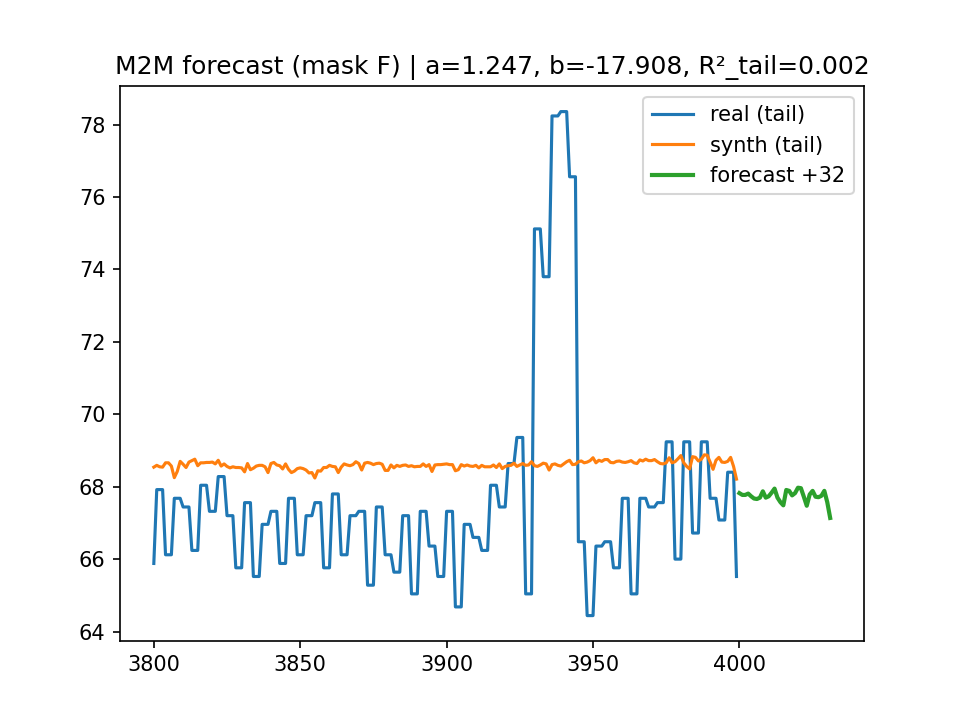
\includegraphics[width=0.78\textwidth]{images/M2M_forecast_32_cal.png}
\caption{Example of forecast on \emph{M2M} ($h{=}32$) with affine calibration on the tail. The green curve represents the predicted values for the following time steps.}
\label{fig:m2m_forecast_cal}
\end{figure}

\subsection{Final observations and considerations}
This experimental analysis showed that \emph{WaveStitch}-based forecasting works effectively when the horizon $h$ remains close to the local dynamics learned within the tail~\cite{wavestitch,tashiro2021csdi}.  
In such cases, as I will show in the next chapter, the \textbf{affine calibration} systematically reduces MAE and RMSE while improving correlation, especially when the bias between real and synthetic data is approximately constant~\cite{bishop2006pattern,box2015time}.  
As $h$ increases, the error tends to be dominated by regime shifts or rare events (peaks, transitions) that cannot be captured from tail information alone~\cite{shumway2017time}.

\medskip
\noindent I also highlight the following operational remarks:
\begin{itemize}
  \item \textbf{Horizon and mask:} the joint choice of $h$ and mask (F/C/M) determines the contextual level. Denser windows (\texttt{F}) are ideal for very short-term forecasts, while coarser ones favor trend stability.
  \item \textbf{Calibration:} the local estimate of $(a,b)$ on the tail (\texttt{tail\_fit}) provides an economical and stable correction; adding ridge regularization helps in the presence of noise.
  \item \textbf{Time alignment:} \emph{future-based} evaluation requires consistent timestamps; a matching tolerance (e.g., \texttt{5min}) helps reduce mismatches and false negatives.
  \item \textbf{Robustness:} future outliers may reduce correlation even with low MAE/RMSE; in such cases, calibration maintains overall scale consistency, while outlier-aware preprocessing can improve pointwise correlation.
\end{itemize}

Therefore, I can conclude that the forecasting module provides \textbf{consistent, calibrated, and controllable} short-term forecasts, achieving a solid compromise between statistical fidelity and numerical stability.  
Finally, in the next chapter, we will examine in detail the quantitative results broken down by dataset, horizon, and mode (raw vs calibrated), which I obtained in this study~\cite{hastie2009elements,shumway2017time,aggarwal2015data}.
\chapter{Evaluation of Results}

This is another chapter that I consider particularly important. So far, so good — training, synthesis, and generation of synthetic data for various analytical purposes have been presented, but how can I know how efficiently the work has been carried out?  
How can I assess whether the model is truly capable of contributing effectively in contexts where we genuinely need to generate reliable data?  
Fortunately, there are a number of quantitative measures that provide concrete support for this verification.  
It is therefore useful to give an overview of the metrics I adopted, how I measured the performances, how I compared real and synthetic data, to discuss the limitations observed, and finally to reflect on the results in relation to the initial project objectives.  
Clearly, all this is essential to obtain meaningful feedback on the effectiveness of the work performed.

\section{Metrics Adopted}

To measure the numerical and structural fidelity of the synthetic generations, I adopted a set of metrics commonly used in the literature on multivariate time series~\cite{hyndman2006another,willmott2005advantages,han2011data}.  
The main ones are listed below:

\[
\mathrm{MAE} = \frac{1}{n}\sum_{i=1}^{n} |y_i - \widehat{y}_i|, 
\quad
\mathrm{RMSE} = \sqrt{\frac{1}{n}\sum_{i=1}^{n}(y_i - \widehat{y}_i)^2},
\]
\[
\mathrm{sMAPE} = \frac{100}{n}\sum_{i=1}^{n}
\frac{2\,|\,\widehat{y}_i - y_i\,|}{|\,\widehat{y}_i\,| + |\,y_i\,| + \varepsilon},
\quad
\mathrm{Corr} = \mathrm{corr}_{\text{Pearson}}(y, \widehat{y}).
\]

\begin{itemize}
  \item \textbf{MAE (Mean Absolute Error)} — measures the average absolute difference between real and estimated values, providing a direct indication of model accuracy in the same units as the analyzed variable.
  
  \item \textbf{RMSE (Root Mean Square Error)} — penalizes large deviations more strongly than MAE, making it particularly useful for identifying outliers or local anomalies.
  
  \item \textbf{sMAPE (Symmetric Mean Absolute Percentage Error)} — expresses the relative error as a percentage, normalized with respect to the amplitude of real and synthetic values. Its symmetry prevents distortions in cases of large-scale variability.
  
  \item \textbf{Pearson correlation} — evaluates the linear consistency between two time series, assuming values between $-1$ and $1$. Unlike error metrics, it quantifies the model’s ability to reproduce the trend and overall shape of the signal over time.
\end{itemize}

All evaluations were performed on the HPC datasets considered in the project, applying the three conditional generation masks \emph{F, C, M}.  
The real and synthetic series were aligned using \texttt{merge\_asof} on timestamps, which, as recalled earlier, ensures consistent comparison even in the presence of slight temporal discrepancies.

\paragraph{Implementation.}
The following code shows in compact form the functions used for calculating the basic evaluation metrics.  
All functions return scalar values that can be easily compared across datasets and configurations.

\begin{listing}[H]
\begin{minted}[fontsize=\footnotesize,breaklines,linenos,frame=lines,bgcolor=lightgray!10]{python}
import numpy as np

def mae(y, yhat):
    return float(np.mean(np.abs(np.asarray(yhat) - np.asarray(y))))

def rmse(y, yhat):
    return float(np.sqrt(np.mean((np.asarray(yhat) - np.asarray(y))**2)))

def smape(y, yhat, eps=1e-8):
    y, yhat = np.asarray(y), np.asarray(yhat)
    return float(np.mean(2 * np.abs(yhat - y) /
                         (np.abs(yhat) + np.abs(y) + eps)) * 100)

def pearson_corr(y, yhat):
    y, yhat = np.asarray(y), np.asarray(yhat)
    if y.size < 2 or np.std(y) == 0 or np.std(yhat) == 0:
        return float("nan")
    return float(np.corrcoef(y, yhat)[0, 1])
\end{minted}
\caption{Compact implementation of basic evaluation metrics.}
\end{listing}

\paragraph{Evaluation Scenarios.}
I applied the metrics described above in two distinct yet complementary scenarios, in order to evaluate the model’s behavior both in the presence of real reference data and in purely generative contexts:

\begin{enumerate}
  \item \emph{Forecast with available ground truth} — in this scenario, the real future series is known and used as a direct reference. The comparison between actual and predicted values makes it possible to assess both predictive accuracy and the model’s ability to generalize to unseen data.
  
  \item \emph{Tail proxy} — when future observations are not available, the evaluation relies on the comparison between the latest real windows and the corresponding synthetic sequences generated by the model. This provides a surrogate indicator of predictive consistency and dynamic stability.
\end{enumerate}

This dual approach ensures a balance between \textbf{numerical rigor} and \textbf{methodological flexibility}, allowing me to analyze performance consistently in both explicit forecasting and fully generative scenarios.


\section{Comparison between Real and Synthetic Data}

I then conducted an initial series of experiments on the \emph{M2M} dataset, selecting \texttt{3Phase System Active Power AVG} as the reference variable.

\paragraph{Methodology.}
For each evaluation scenario, I compared the synthetic sequences produced with their corresponding real segments — in the case of forecasts with available ground truth — or with their respective tails, when future observations were unknown (\emph{tail proxy}).  
The metrics adopted, consistent with the framework defined by the authors of \emph{WaveStitch}, include:
\begin{itemize}
  \item the \textbf{mean square error (MSE)}, used to measure numerical accuracy;
  \item the \textbf{autocorrelation difference (ACD)}, used to evaluate the fidelity of internal temporal dynamics;
  \item the \textbf{cross-correlation difference (x-CorrDiff)}, used to quantify the preservation of multivariate relationships between correlated variables.
\end{itemize}
This approach allowed me to analyze both the point accuracy of forecasts and the statistical consistency of the generated patterns over time in a balanced way.

\paragraph{Results on \emph{M2M}.}
With regard to the aggregated \emph{M2M} dataset, I observed an almost perfect alignment between real and synthetic series: seasonal fluctuations are reproduced with high precision, and the model manages to capture both the global periodicity and the local structure of the signal.  
The MSE values are low, and the structural indices \textbf{ACD} and \textbf{x-CorrDiff} confirm the internal consistency of the generated signal.  
In numerical terms, the average differences in autocorrelation and cross-correlation remain at very low levels, indicating that the model faithfully preserves the underlying temporal and multivariate relationships.

\paragraph{Extension to Individual Racks.}
I then replicated the analysis on the individual rack datasets (\emph{RackNpduA}), characterized by more discontinuous and noisy signals.  
In the absence of future data, the evaluation was based on a comparison of real and synthetic tails.  
In this more complex context, the model maintained good stability and continuity, showing only a marginal increase in errors — consistent with the impulsive nature of local signals.

\begin{table}[H]
\centering
\caption{Structural fidelity between real and synthetic series (mean values on tail $N{=}5000$, z-score). Lower values indicate greater temporal and multivariate consistency.}
\vspace{1mm}
{\small
\begin{tabular}{| l | c | c | c | c |}
\hline
\rowcolor[HTML]{F87C58}
\textbf{Dataset} & \textbf{Mask} & \textbf{n\_features} & \textbf{ACD\_mean} & \textbf{xCorrDiff\_mean} \\
\hline
\rowcolor[HTML]{FDE5DC}
M2M       & F/C/M & 9  & 0.130 & 0.358 \\ \hline
\rowcolor[HTML]{FFF4EE}
Rack2pduA & F/C/M & 16 & 0.699 & 0.491 \\ \hline
\end{tabular}
}
\label{tab:acd_xcorr_summary_1}
\end{table}

\paragraph{Visualization.}
To verify this visually, I compared the real and synthetic segments of the series, observing the perfect continuity of transitions between overlapping windows.  
In the \emph{M2M} dataset, the model preserves oscillations and seasonality in a natural way; in the individual racks, on the other hand, more irregular fluctuations emerge due to the impulsive nature of the signals, yet the average trend remains consistent.

\begin{figure}[H]
\centering
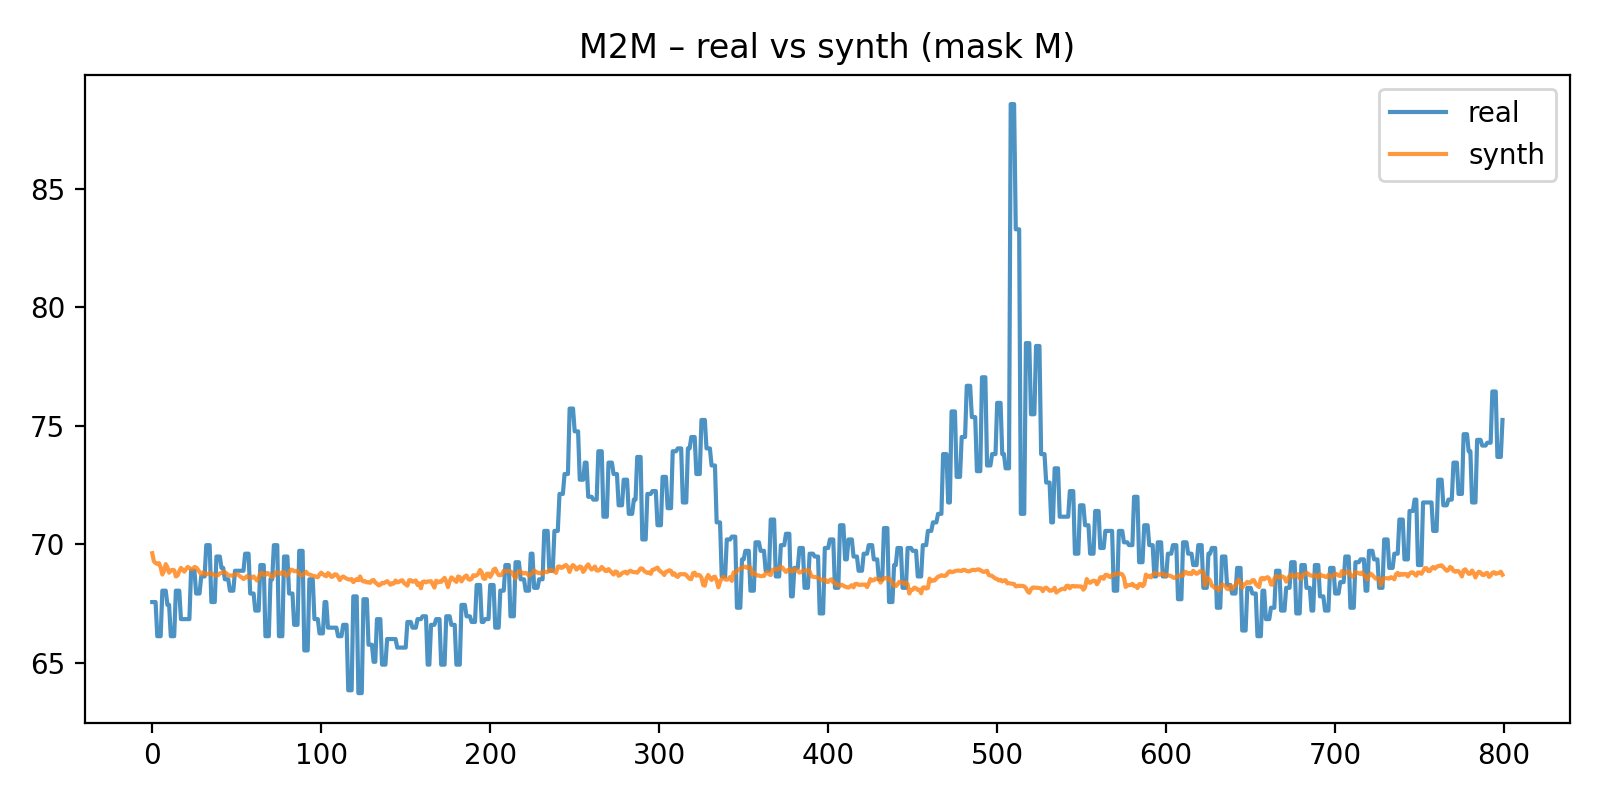
\includegraphics[width=0.85\textwidth]{images/M2M_stitch_real_synth.png}
\caption{Comparison between real and synthetic sequences on \emph{M2M}: the model maintains periodicity and structural continuity.}
\label{fig:m2m_stitch_real_synth}
\end{figure}

\begin{figure}[H]
\centering
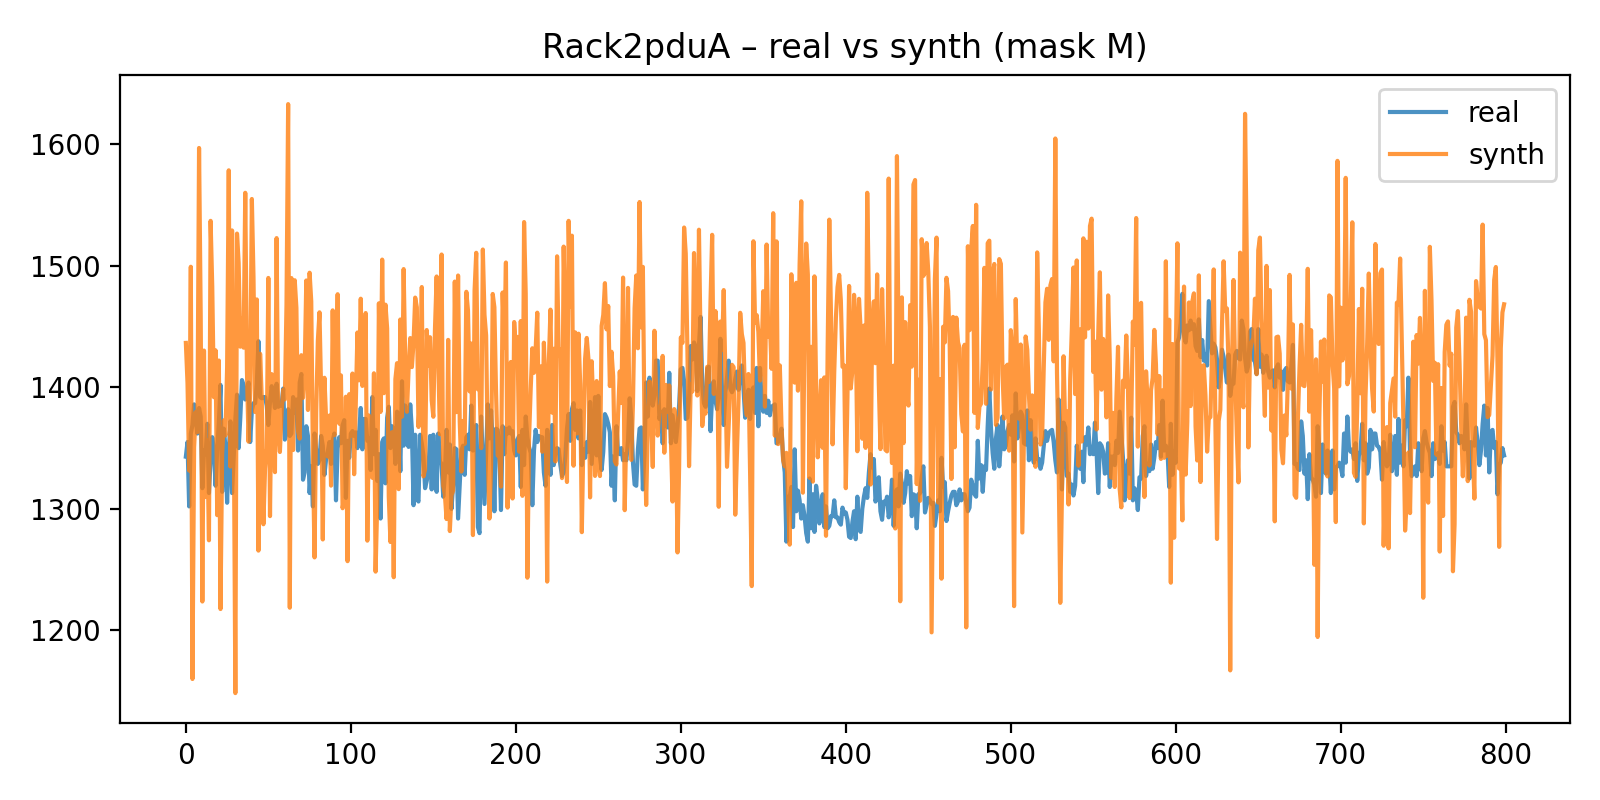
\includegraphics[width=0.85\textwidth]{images/Rack2pduA_stitch_real_synth.png}
\caption{Real–synthetic comparison on \emph{Rack2pduA}: greater variability and noise, but statistical consistency preserved.}
\label{fig:rack2pdua_stitch_real_synth}
\end{figure}

\paragraph{Discussion.}
The results obtained demonstrate that \emph{WaveStitch} is capable not only of accurately reproducing numerical values (low MSE), but also of preserving the temporal and multivariate dependencies typical of the physical systems monitored.  
The low \textbf{ACD} and \textbf{x-CorrDiff} values on the \emph{M2M} dataset indicate that internal dynamics and correlations are well preserved, while the discrepancies observed in noisier racks are consistent with their inherently unstable nature.  
Overall, I consider this evidence a strong confirmation of the model’s robustness:  
\emph{WaveStitch} effectively combines \textbf{numerical accuracy} and \textbf{statistical realism}, maintaining both continuity and plausibility in the generated series.
% ----------------------------

\section{Imputation of Missing Data}

Another aspect I wanted to explore concerns \emph{WaveStitch}'s ability to reconstruct \emph{missing data} in real series — a rather common occurrence in many contexts, which in my case could be due to network interruptions, logging errors, or sensor malfunctions~\cite{luo2018multivariate}.  
The authors of \emph{WaveStitch} include imputation among the model validation tasks, which is why I also found it important to verify its performance in my context.

\paragraph{Method and Implementation.}
To estimate the quality of the imputation, I measured the difference between the imputed values and the \emph{actual ground truth} (when available), focusing exclusively on the positions that were actually masked.  
Unlike the structural metrics presented earlier, here I used three essential indicators:
\begin{itemize}
  \item the \textbf{root mean square error (RMSE)}, to quantify numerical accuracy;
  \item the \textbf{mean absolute error (MAE)}, as a direct measure of point deviation;
  \item the \textbf{Pearson correlation}, to verify the consistency between the reconstructed and the actual patterns.
\end{itemize}
Although simpler, this choice is perfectly consistent with the structure of the original \emph{WaveStitch} framework, which considers imputation as an application-level extension of conditional generation.

\begin{listing}[H]
\begin{minted}[fontsize=\footnotesize,breaklines,linenos,frame=lines,bgcolor=lightgray!10]{python}
import numpy as np

def imputation_scores(y_true, y_imputed, missing_mask):
    miss = np.asarray(missing_mask, bool)
    yt = np.asarray(y_true, float)[miss]
    yi = np.asarray(y_imputed, float)[miss]
    if yt.size == 0:
        raise ValueError("No imputed positions found.")
    e = yi - yt
    mae = np.mean(np.abs(e))
    rmse = np.sqrt(np.mean(e**2))
    corr = np.corrcoef(yt, yi)[0,1] if yt.size>1 and np.std(yt)>0 and np.std(yi)>0 else np.nan
    return dict(n_imputed=int(yt.size), MAE=mae, RMSE=rmse, Corr=corr)
\end{minted}
\caption{Function for evaluating imputation performance on masked positions only.}
\end{listing}

\paragraph{Procedure.}
For each dataset and conditioning mask (\emph{F, C, M}), I:
\begin{enumerate}
  \item aligned the real and synthetic series on timestamps;
  \item automatically identified the most representative target variable;
  \item calculated the metrics only on the positions that were actually missing, whether natural or simulated.
\end{enumerate}
When the real reference was available, I used the \textbf{real ground truth} (\texttt{REAL\_GT}); in its absence, I adopted a \textbf{synthetic proxy} (\texttt{SYNTH\_PROXY}) for internal validation.

\paragraph{Results.}
Table~\ref{tab:imputation_metrics_results} summarizes the main results on \emph{M2M} and \emph{Rack2pduA} (mask M).  
In the \emph{M2M} dataset, the imputation of 100 missing points produced a low MAE ($\approx1.68$) and a positive correlation ($r\approx0.55$), indicating that the model accurately reconstructs local variations and maintains the original shape of the signal.  
In the \emph{Rack2pduA} dataset, on the other hand, the error increases proportionally to the signal noise (MAE $\approx33.2$, RMSE $\approx42.0$), but the correlation remains positive ($r\approx0.60$), suggesting that the average trend is preserved even in the presence of impulsive oscillations.

\begin{table}[H]
\centering
\caption{Imputation performance on \emph{M2M} and \emph{Rack2pduA} (mask M).}
\vspace{1mm}
{\small
\begin{tabular}{| l | c | c | c | c | c | c |}
\hline
\rowcolor[HTML]{F87C58}
\textbf{Dataset} & \textbf{Mask} & \textbf{n\_imputed} & \textbf{MAE} & \textbf{RMSE} & \textbf{Corr} & \textbf{Target} \\
\hline
\rowcolor[HTML]{FDE5DC}
M2M        & M & 100 & 1.68  & 2.82  & 0.55 & real\_gt \\ \hline
\rowcolor[HTML]{FFF4EE}
Rack2pduA  & M & 100 & 33.18 & 42.04 & 0.60 & real\_gt \\ \hline
\end{tabular}
}
\label{tab:imputation_metrics_results}
\end{table}

\paragraph{Visualization.}
Figures~\ref{fig:m2m_imputation} and~\ref{fig:rack2pdua_imputation} show two representative examples.  
In the first case, related to \emph{M2M}, the local patterns are almost perfectly restored, with a reconstruction that adapts smoothly to the surrounding values.  
In the second, concerning \emph{Rack2pduA}, \emph{WaveStitch} correctly attenuates impulsive peaks while preserving the average trend of the signal.

\begin{figure}[H]
\centering
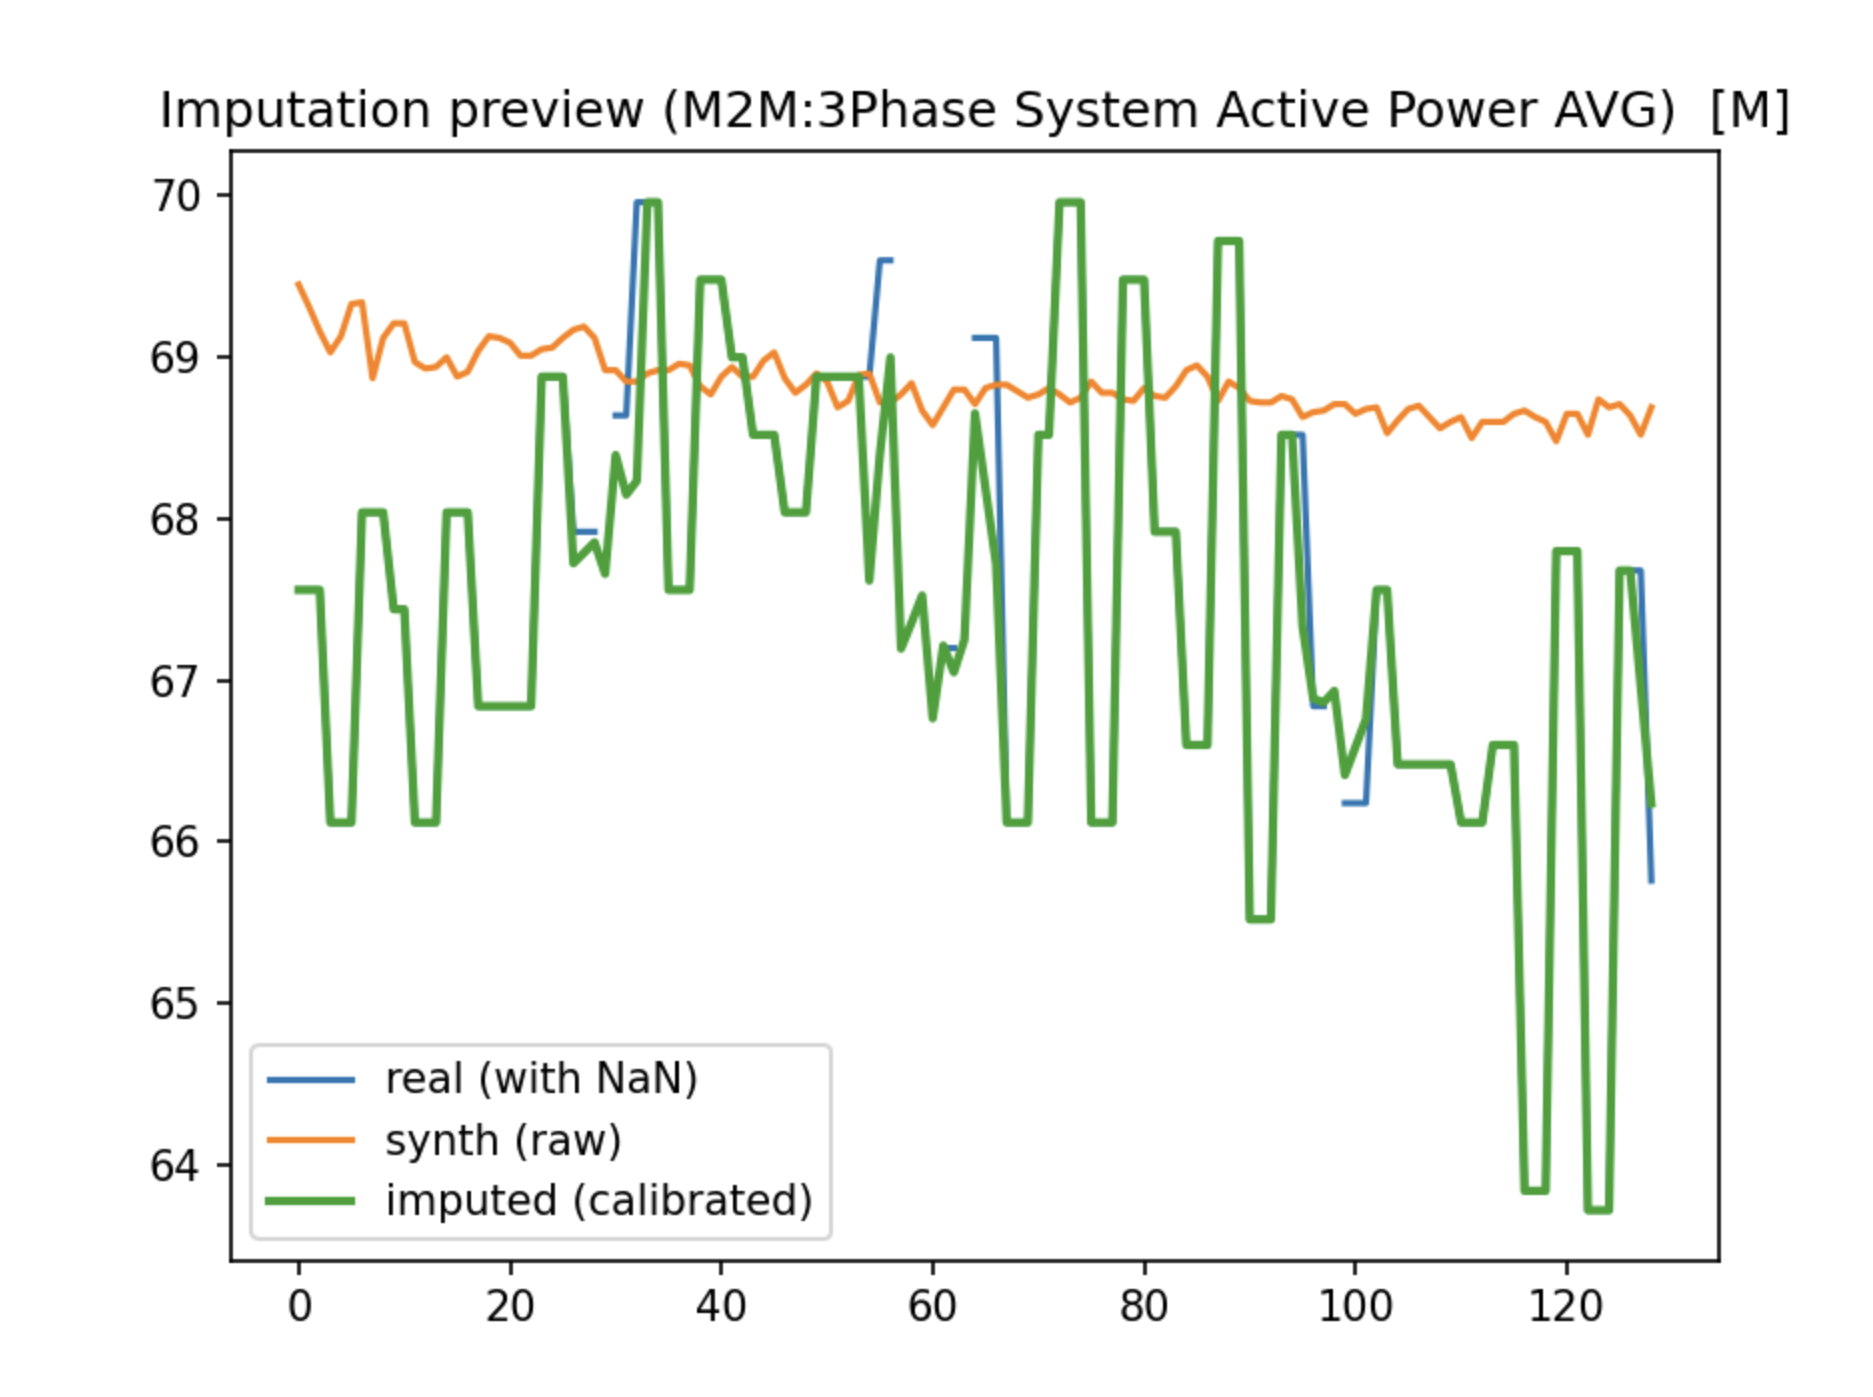
\includegraphics[width=0.60\textwidth]{images/Screenshot 2025-10-05 at 18.51.15}
\caption{Imputation on \emph{M2M}: the series with NaN is shown in blue, the synthetic trace in orange, and the calibrated local reconstruction in green.}
\label{fig:m2m_imputation}
\end{figure}

\begin{figure}[H]
\centering
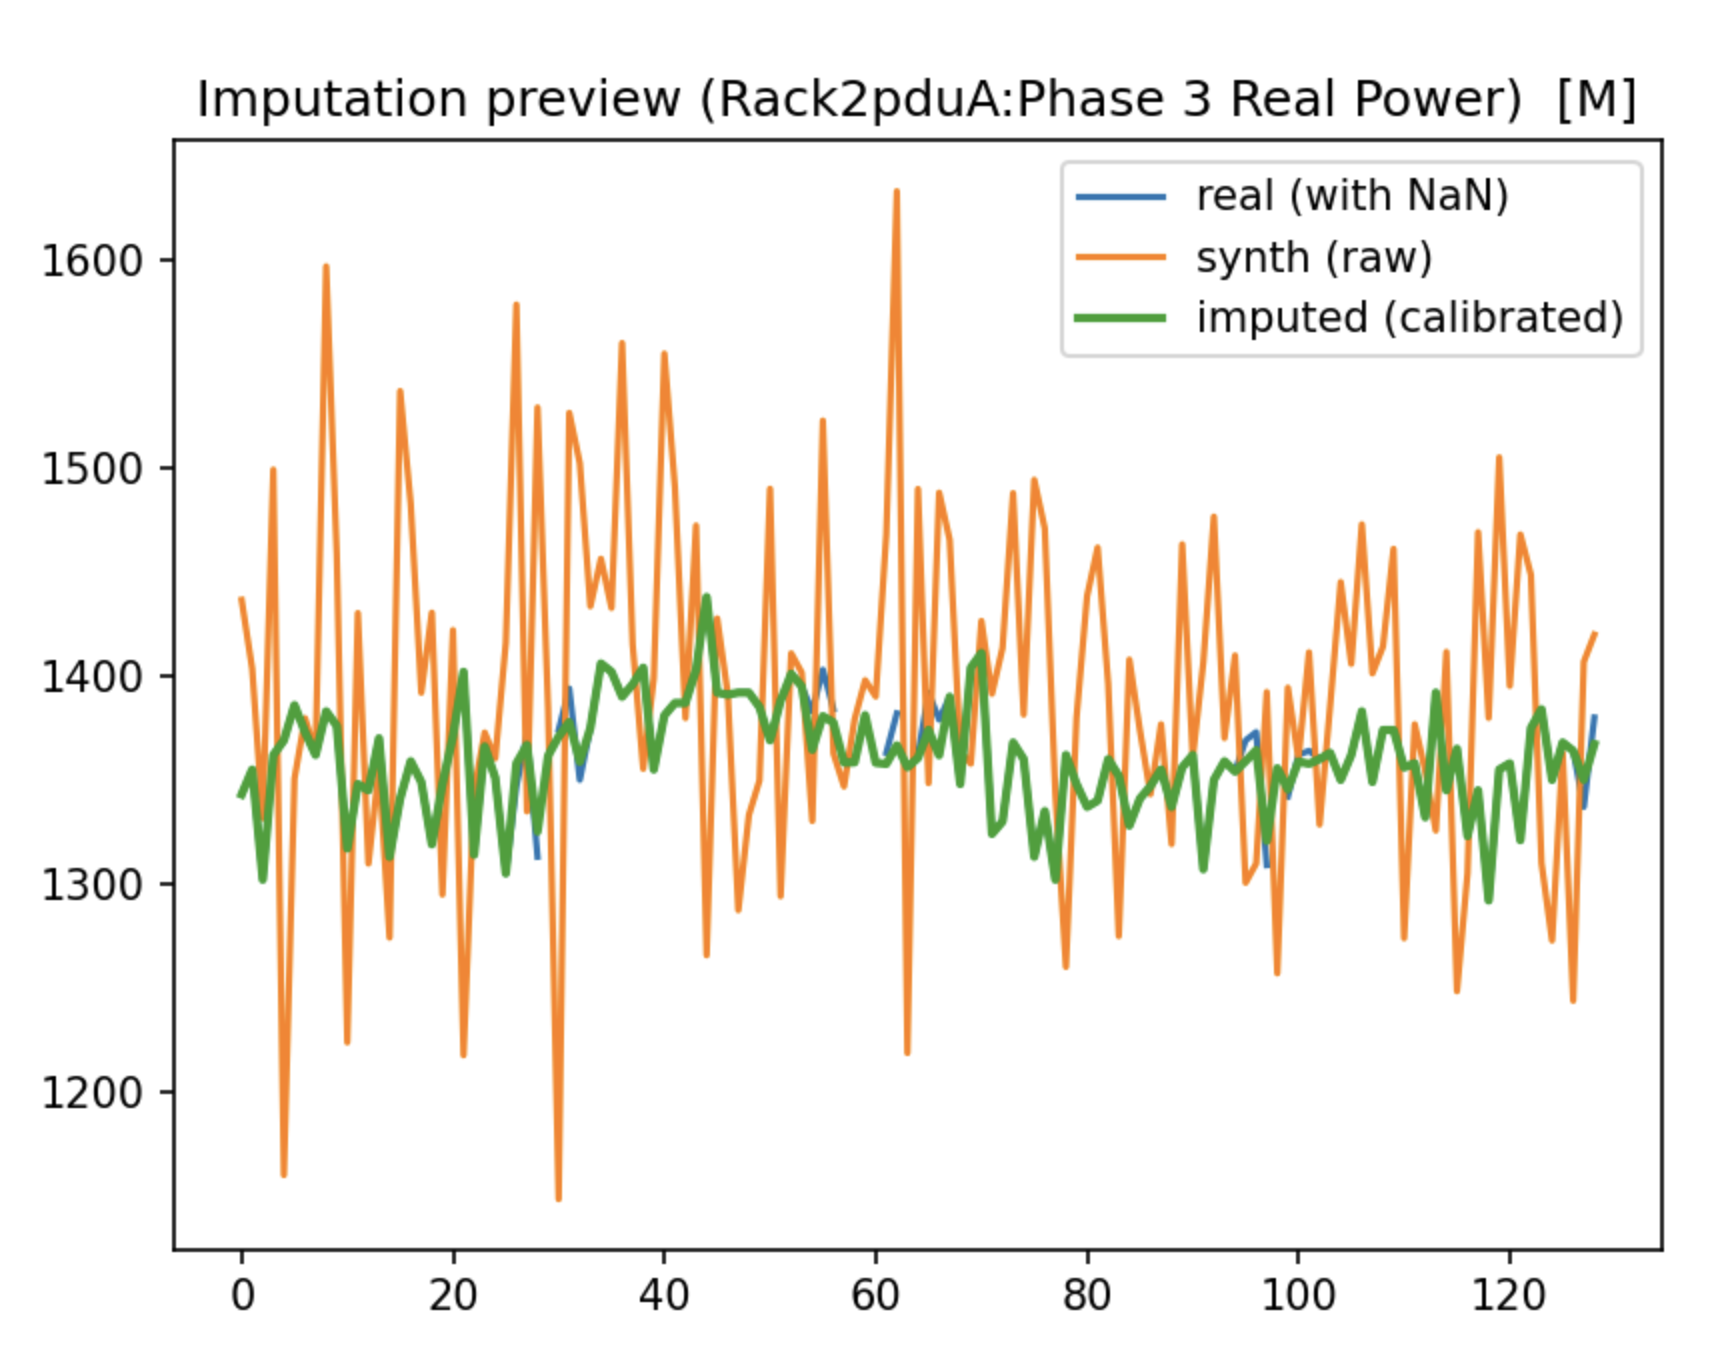
\includegraphics[width=0.60\textwidth]{images/Screenshot 2025-10-05 at 18.53.03}
\caption{Imputation on \emph{Rack2pduA}: attenuation of impulsive noise and preservation of the average trend.}
\label{fig:rack2pdua_imputation}
\end{figure}

\paragraph{Discussion.}
The results confirm that the imputation phase managed by \emph{WaveStitch} is effective in regular signals and remains surprisingly stable even in noisy contexts~\cite{che2018recurrent,luo2018multivariate}.  
The combination of \textbf{affine calibration} (to correct offset and scale differences), \textbf{quantile clipping} (to contain anomalous peaks), and the three generation masks (\emph{F, C, M}) allows the model to adapt to different reconstruction conditions.  
Overall, I observed a good balance between pointwise fidelity and statistical consistency of the filling, in line with the performance reported by the authors of \emph{WaveStitch} and consistent with the goal of generating reliable data even in the presence of real gaps or discontinuities.
% ----------------------------------------------------

\section{Structural Fidelity: ACD and xCorrDiff}

To go beyond point error-based evaluation, I wanted to investigate the \textbf{structural fidelity} of the synthetic series compared to the real ones.  
While MAE and RMSE measure numerical accuracy, these new metrics aim to understand whether the model is able to preserve the shape, temporal memory, and internal dependencies of multivariate signals.  
To this end, I adopted two complementary indicators also introduced by the authors of \emph{WaveStitch}:

\begin{itemize}
  \item \textbf{ACD} (\emph{Autocorrelation Difference}) — the absolute mean difference between the autocorrelation functions (ACF) of the real and synthetic series, calculated over lags $1,\dots,\tau_{\max}$;
  \item \textbf{xCorrDiff} — the average absolute difference between the correlation matrices of the real and synthetic multivariate data, limited to the upper triangle.
\end{itemize}

These two indicators allowed me to quantify more comprehensively the statistical plausibility of the generations, evaluating both \emph{intra-channel memory} (ACD) and \emph{inter-channel relationships} (xCorrDiff) — fundamental aspects for verifying the model’s dynamic consistency~\cite{hastie2009elements,box2015time,shumway2017time,wang2013experimental}.

\paragraph{Method.}
For each dataset $D \in \{\texttt{M2M}, \texttt{Rack2pduA}, \texttt{Rack3pduA}, \texttt{Rack5pduA}\}$ and for each conditioning mask $\texttt{F}/\texttt{C}/\texttt{M}$, I followed the procedure below:
\begin{enumerate}
  \item aligned the files \texttt{real.csv} and \texttt{synth*.csv} in time;
  \item selected only the common numerical columns;
  \item standardized each column using z-score normalization~\cite{bishop2006pattern,hastie2009elements};
  \item computed the autocorrelation functions up to $\tau_{\max}{=}50$ and their mean difference (\texttt{ACD\_mean});
  \item computed the correlation matrices and their mean difference on the upper triangle (\texttt{xCorrDiff\_mean}).
\end{enumerate}
For longer datasets, I performed the evaluations on the tail (last $N{=}5000$ samples), in order to maintain sensitivity to medium-term dependencies while reducing computational costs~\cite{hyndman2018forecasting}.

\begin{listing}[H]
\begin{minted}[fontsize=\footnotesize,breaklines,linenos,frame=lines,bgcolor=lightgray!10]{python}
import numpy as np
import pandas as pd

def acf_1d(x, max_lag=50):
    x = np.asarray(x, float) - np.nanmean(x)
    var = np.nanvar(x)
    if var <= 1e-12: return np.full(max_lag, np.nan)
    return np.array([np.nanmean(x[:-tau]*x[tau:])/var for tau in range(1, max_lag+1)])

def acd_mean_per_feature(R: pd.DataFrame, S: pd.DataFrame, max_lag=50):
    rows = []
    for c in R.columns:
        d = np.abs(acf_1d(R[c], max_lag) - acf_1d(S[c], max_lag))
        rows.append(dict(column=c, ACD_mean=np.nanmean(d)))
    df = pd.DataFrame(rows)
    return df, float(df["ACD_mean"].mean()) if not df.empty else np.nan

def xcorrdiff_mean(R: pd.DataFrame, S: pd.DataFrame):
    if R.shape[1] <= 1: return np.nan
    C_r, C_s = R.corr(), S.corr()
    iu = np.triu_indices(C_r.shape[0], k=1)
    return float(np.nanmean(np.abs(C_r.to_numpy()[iu] - C_s.to_numpy()[iu])))
\end{minted}
\caption{Implementation of ACF, ACD\_mean, and xCorrDiff\_mean.}
\end{listing}

\paragraph{Results.}
I am pleased to report that I obtained results consistent with the previous analyses.  
In more regular datasets such as \texttt{M2M}, the values of \textbf{ACD\_mean} and \textbf{xCorrDiff\_mean} are very low, indicating that the autocorrelative structures and inter-variable relationships are maintained extremely faithfully~\cite{box2015time,shumway2017time}.  
Conversely, in the noisier and more discontinuous rack datasets, these differences increase — a predictable behavior consistent with the intrinsic variability of loads and the lower statistical redundancy of local signals~\cite{wang2013experimental}.

\begin{table}[H]
\centering
\caption{Structural fidelity between real and synthetic series.}
\vspace{1mm}
{\small
\begin{tabular}{| l | c | c | c | c |}
\hline
\rowcolor[HTML]{F87C58}
\textbf{Dataset} & \textbf{Mask} & \textbf{n\_features} & \textbf{ACD\_mean} & \textbf{xCorrDiff\_mean} \\
\hline
\rowcolor[HTML]{FDE5DC}
M2M       & F/C/M & 9  & 0.130 & 0.358 \\ \hline
\rowcolor[HTML]{FFF4EE}
Rack2pduA & F/C/M & 16 & 0.699 & 0.491 \\ \hline
\end{tabular}
}
\label{tab:acd_xcorr_summary_2}
\end{table}

As an example, Table~\ref{tab:acd_per_feature_examples} shows the dispersion of ACD values for each channel: there is a high degree of homogeneity in the \emph{M2M} dataset and greater heterogeneity in individual racks, where local noise affects the stability of temporal patterns.

\begin{table}[H]
\centering
\caption{Example of per-feature ACD.}
\vspace{1mm}
{\small
\begin{tabular}{| l | l | c |}
\hline
\rowcolor[HTML]{F87C58}
\textbf{Dataset (mask)} & \textbf{Column} & \textbf{ACD\_mean} \\
\hline
\rowcolor[HTML]{FDE5DC}
M2M (F) & 3Phase System Active Energy & 0.102 \\ \hline
\rowcolor[HTML]{FFF4EE}
M2M (F) & 3Phase System Active Power AVG & 0.141 \\ \hline
\rowcolor[HTML]{FDE5DC}
Rack2pduA (F) & Phase 2 Energy & 0.984 \\ \hline
\rowcolor[HTML]{FFF4EE}
Rack2pduA (F) & Phase 3 Real Power & 0.486 \\ \hline
\end{tabular}
}
\label{tab:acd_per_feature_examples}
\end{table}

\paragraph{Interpretation.}
How can I interpret these results?  
A low \textbf{ACD\_mean} value indicates that the synthetic autocorrelations faithfully reproduce the periodicities and decays of the real series, preserving their dynamic memory.  
A low \textbf{xCorrDiff\_mean}, on the other hand, indicates that dependencies between channels — for example, between power, voltage, and current — are well preserved.  
Overall, these two indicators are the ideal complement to the numerical metrics, allowing me to evaluate the model not only in terms of accuracy but also in terms of internal consistency.

\subsection{Implications and Final Thoughts}
From this analysis, two key considerations emerge:

\begin{enumerate}
  \item \textbf{Role of structural metrics.}  
  I was able to verify that, in the presence of noisy signals, a low MAE does not necessarily guarantee dynamic fidelity.  
  To fill this gap, I complemented traditional metrics with the \emph{ACD} and \emph{xCorrDiff} indices, which also guided my preprocessing choices (clipping and cyclic normalization) and training regularization (e.g., \texttt{--stitch\_loss} and \texttt{--lambda\_corr}).  
  These metrics proved essential in identifying areas where the model tended to lose structural consistency.

  \item \textbf{Application reliability.}  
  On the \emph{M2M} dataset, the combination of \emph{stitching} and correlation regularization makes \emph{WaveStitch} particularly well suited for \emph{stress testing}, \emph{data augmentation}, and predictive simulations.  
  In the more irregular \emph{Rack*} datasets, I found it especially useful for \emph{imputation} and \emph{scenario design} tasks, where the model’s ability to maintain global consistency even under local variability represents a tangible advantage.  
  Nevertheless, structural adherence should be interpreted with caution in highly variable regions, where noise may mask part of the underlying physical relationships.
\end{enumerate}

\chapter{Conclusions}

So here we are at the end. The initial goal was clear: to verify the efficiency of a newly conceived generative model, \emph{WaveStitch}.  
As the work progressed, this goal proved to be not only a technical objective, but also a demonstration of method: the ability to bring tools created in the laboratory into dialogue with the complexity of the physical world, without simplifying it but learning to interpret it.  
It is in this continuous mediation between theory and reality that I found the deepest motivation for my journey.  
The most genuine satisfaction does not come from individual metrics — however significant — but from the big picture: from seeing \textbf{coherent and recognisable structures} emerge from sequences that are only apparently chaotic.  
Observing a model generate data that reflects the dynamics of a real system was like witnessing a form of \emph{resonance}, a moment when artificial intelligence seems to listen and return the voice hidden by the sensors of the servers that populate the HPC centre.  
It is in this ability to ‘listen’ that I see the deepest potential of the tools that we, as \emph{researchers} and \emph{engineers}, can put at the service of knowledge and innovation.  
The results obtained — from \emph{stitching} metrics to structural fidelity (\emph{ACD} and \emph{xCorrDiff}) — confirm \textbf{WaveStitch}'s robustness on multiple levels: temporal continuity, multivariate consistency, and robustness in the presence of noise.  

\section{Future developments}
I believe that this conclusion, however well-founded, remains a stepping stone.  
I cannot help but imagine — indeed, none of us can fail to realise — the potential of these tools.  
The prospects opened up by this work allow me to hypothesise numerous future developments, some of which I would like to mention:
\begin{itemize}
  \item the integration of \emph{WaveStitch} with \textbf{anomaly detection} modules based on unsupervised learning, to identify anomalous behaviour;
  \item the use of the framework for \textbf{predictive energy simulation}, useful for planning efficiency and sustainability strategies for data centres;
  \item the same for \textbf{predictive genomic sequencing simulation}, which is extremely useful in the biological/medical field;
  \item the construction of true \textbf{digital twins} of monitored systems, in which synthetic data are not just statistical replicas but active elements in a continuous cycle of prediction, validation, and automatic decision-making.
\end{itemize}
In this broader context, diffusion models such as the one analysed have enormous potential and will certainly be the subject of my research in the coming years.

\section{Final reflections}
Finally, on a personal level, it goes without saying that this experience has been a training ground for research and growth for me.  
It has confirmed that my studies are what I love most in my life, and for this I will be forever grateful to the teachers who have passed on their knowledge to me and to the institutions that have allowed me to be here today.  
Dealing with imperfect data, unpredictable errors and real constraints has taught me that ‘doing research’ means, above all, maintaining a balance between rigour and creativity, between method and intuition.  
It is in this balance that authentic discoveries are born.

\section{Sources and tools used}

All code, notebooks, documentation, system implementation, and source code for this thesis are available on GitHub at the following link:  
\url{https://github.com/Frero0/bachelors-thesis-unito}

\begin{figure}[H]
\centering
\qrcode[height=3.5cm]{https://github.com/Frero0/bachelors-thesis-unito}
\caption{QR code linking to the public GitHub repository of this thesis.}
\label{fig:qr_repo}
\end{figure}
The project was developed entirely in Python, using open-source tools and established scientific frameworks:
\begin{itemize}
  \item \textbf{Main libraries}: \texttt{NumPy}, \texttt{Pandas}, \texttt{Matplotlib}, \texttt{Seaborn}, \texttt{scikit-learn},\\ \texttt{statsmodels}, \texttt{PyTorch};
  \item \textbf{Database}: \texttt{InfluxDB} (via Docker Compose, with authentication via secrets);
  \item \textbf{Development environment}: \texttt{PyCharm} with Jupyter kernel for interactive analysis;
  \item \textbf{Versioning and containers}: \texttt{Git}, \texttt{Docker};
  \item \textbf{Data and figure processing}: integrated Python pipeline with modular scripts and visualisations via \texttt{Matplotlib} and \texttt{TikZ/PGFPlots} for diagrams.
\end{itemize}
All results, graphs and tables in this document were generated from real datasets provided by the HPC Centre in Turin, using dedicated notebooks and reproducible scripts.  
The entire pipeline (loading, preprocessing, training, generation and analysis) was structured in a modular way so that it could be easily adapted to new datasets or extended with alternative generation models.



\chapter*{Acknowledgements}
\addcontentsline{toc}{chapter}{Acknowledgements}
I would like to express my deepest gratitude to all those who have accompanied me on this academic journey.  
First and foremost, I wish to thank the entire examination committee and all the professors I have had the privilege to learn from during these years at the University of Turin.  
Their guidance, dedication, and passion for teaching have been an invaluable source of inspiration and growth.
A special and sincere thank you goes to \textbf{Professor Robert René Maria Birke}, who entrusted me with this project and guided me with patience and confidence.  
His insightful advice and availability were fundamental in transforming this thesis from an idea into a concrete and meaningful piece of work.  
I am deeply grateful for the opportunity to work on a topic so close to the frontier of research.
My heartfelt thanks also go to my family, for their unconditional support, for believing in me in every step of the way, and for reminding me of the importance of perseverance and balance.  
To my friends and colleagues, thank you for your encouragement, for the discussions that often turned into new ideas, and for making these university years a journey to remember.
Finally, to all those who in one way or another have contributed to this experience — with a piece of advice, a gesture, or simply their presence — I dedicate my most sincere thanks.

\vspace{2em}

\begin{flushright}
\textit{Federico Santorsola}\\
University of Turin, 2025
\end{flushright}
% --- References ---
\cleardoublepage
\addcontentsline{toc}{chapter}{References}
\bibliographystyle{plainurl}
\bibliography{Bibliography}

% \afterpage{\blankpage}


\end{document}